\documentclass[12pt,a4paper]{article}

% --- Cài đặt cơ bản ---
\usepackage[utf8]{inputenc} % Hỗ trợ gõ tiếng Việt
\usepackage[T5]{fontenc}    % Mã hóa font cho tiếng Việt
\usepackage[vietnamese]{babel} % Gói hỗ trợ ngôn ngữ tiếng Việt
\usepackage{geometry}       % Điều chỉnh lề trang
\geometry{a4paper, margin=2.5cm, top=3cm, bottom=3cm} % Cài đặt lề chuẩn

% --- Thiết lập headheight để tránh cảnh báo fancyhdr ---
\setlength{\headheight}{15pt}

% --- Gói cho typography và định dạng chuyên nghiệp ---
\usepackage{setspace}       % Điều chỉnh khoảng cách dòng (ví dụ: 1.5 lines)
\usepackage{titlesec}       % Tùy chỉnh định dạng tiêu đề các phần/chương
\usepackage{tocloft}        % Tùy chỉnh mục lục và danh sách bảng/hình
\usepackage{caption}        % Tùy chỉnh caption cho bảng và hình ảnh
\usepackage{subcaption}     % Hỗ trợ subfigure và subcaption (nếu cần nhiều hình trong 1 caption)
\usepackage{ragged2e}       % Cho phép căn đều văn bản (justifying), tốt hơn \justify
\usepackage{booktabs}       % Cho bảng đẹp hơn với đường kẻ chuyên nghiệp (\toprule, \midrule, \bottomrule)
\usepackage{array}          % Hỗ trợ định dạng cột nâng cao (>{\raggedright\arraybackslash}p{width})
\usepackage{enumitem}       % Tùy chỉnh danh sách (itemize, enumerate)
\usepackage{microtype}      % Cải thiện kiểu chữ và căn chữ
\usepackage{pifont}         % Bộ biểu tượng cho bullet tùy chỉnh
\usepackage{float}          % Cho phép vị trí bảng/hình ảnh chính xác hơn [H]
\usepackage{tabularx}       % Bảng có thể tự động điều chỉnh chiều rộng cột
\usepackage{longtable}      % Cho bảng dài trải dài nhiều trang
\usepackage{graphicx}       % Thêm gói này để chèn ảnh

% --- Gói cho toán học (giữ lại nếu có dùng công thức toán) ---
\usepackage{amsmath}        % Các môi trường toán học mở rộng (align, equation, v.v.)
\usepackage{amssymb}        % Các ký hiệu toán học bổ sung

% --- Gói cho header/footer ---
\usepackage{fancyhdr}       % Tùy chỉnh header và footer

% --- Gói cho màu sắc và đồ họa ---
\usepackage{xcolor}         % Định nghĩa và sử dụng màu sắc
\usepackage[most]{tcolorbox} % Tạo khung màu chuyên nghiệp
\usepackage{tikz}           % Vẽ hình và trang trí
\usetikzlibrary{calc}       % Thư viện hỗ trợ tính toán vị trí
\definecolor{darkblue}{RGB}{0,82,155}   % Màu xanh đậm cho tiêu đề
\definecolor{darkgreen}{RGB}{0,128,0}   % Màu xanh lá đậm cho URL

% --- Tuỳ chỉnh danh sách ---
\setlist[itemize]{leftmargin=1cm,label=\textcolor{darkblue}{\small\textbullet}}

% --- Khung nổi bật cho phân tích rủi ro ---
\newtcolorbox{riskbox}{
    colback=white,
    colframe=darkblue,
    fonttitle=\bfseries,
    coltitle=darkblue,
    boxrule=0.5pt,
    arc=2mm,
    left=4pt,
    right=4pt,
    top=4pt,
    bottom=4pt,
}

% --- Cấu hình định dạng tiêu đề ---
% Sử dụng \normalfont để đảm bảo font không bị ảnh hưởng bởi các lệnh trước đó
\titleformat{\section}{\normalfont\Large\bfseries\color{darkblue}}{\thesection}{1em}{}
\titleformat{\subsection}{\normalfont\large\bfseries\color{darkblue}}{\thesubsection}{1em}{}
\titleformat{\subsubsection}{\normalfont\normalsize\bfseries\color{darkblue}}{\thesubsubsection}{1em}{}

% --- Cấu hình spacing tối ưu ---
\onehalfspacing             % Khoảng cách dòng 1.5
\setlength{\parindent}{0.5cm} % Thụt đầu dòng 0.5cm
\setlength{\parskip}{6pt}   % Khoảng cách giữa các đoạn văn
\setlength{\arrayrulewidth}{0.5pt}  % Độ dày đường viền bảng
\renewcommand{\arraystretch}{1.2}   % Khoảng cách dòng trong bảng
\setlength{\tabcolsep}{6pt} % Khoảng cách giữa các cột trong bảng

% --- Cấu hình hyperref (đặt cuối cùng trong preamble) ---
\usepackage{hyperref}
\hypersetup{
    colorlinks=true,        % Màu cho các liên kết
    linkcolor=darkblue,     % Màu của các liên kết nội bộ (mục lục, hình, bảng)
    filecolor=magenta,      % Màu của liên kết đến file cục bộ
    urlcolor=darkgreen,     % Màu của URL
    citecolor=darkblue,     % Màu của các trích dẫn
    pdftitle={Báo cáo giữa kỳ - Dự án Smart Canteen AR}, % Tiêu đề hiển thị trong thuộc tính PDF
    pdfauthor={Nhóm 5 - Trường Đại học Khoa học Tự nhiên TPHCM}, % Tác giả hiển thị trong thuộc tính PDF
    pdfsubject={Dự án Khởi nghiệp Đổi mới Sáng tạo}, % Chủ đề PDF
    pdfkeywords={Smart Canteen, AR, Thực tế tăng cường, Căng tin thông minh}, % Từ khóa PDF
    bookmarksopen=true,     % Mở bookmark khi mở PDF
    bookmarksnumbered=true, % Đánh số bookmark
    pdfstartview={FitH}     % Chế độ xem khi mở PDF (Fit to Width)
}

% --- Xóa định nghĩa title/author vì không cần dùng \maketitle ---

\begin{document}

% --- Trang tiêu đề ---
\begin{titlepage}
    \thispagestyle{empty} % Xóa header/footer cho trang tiêu đề
    \begin{tikzpicture}[remember picture,overlay]
        \draw[color=darkblue,line width=2pt]
            ($(current page.north west)+(0.75cm,-0.75cm)$)
            rectangle
            ($(current page.south east)+(-0.75cm,0.75cm)$);
    \end{tikzpicture}
    \centering           % Căn giữa nội dung trang bìa

    % Có thể thêm logo nếu có (ví dụ: \includegraphics[width=4cm]{../images/logo.png}\\[1cm])
    \vspace*{2cm} % Khoảng trống phía trên

    % Nội dung tiêu đề được viết trực tiếp thay vì dùng \maketitle
    {\huge\textbf{\color{darkblue}BÁO CÁO GIỮA KỲ}} \\[0.8cm]
    {\LARGE\textbf{\color{darkblue}DỰ ÁN SMART CANTEEN AR}} \\[0.5cm]
    {\large\textit{Ứng dụng thực tế tăng cường trong căng tin thông minh}} \\[1.5cm]

    % Nội dung tác giả được viết trực tiếp
    \textbf{\large BÁO CÁO ĐỒ ÁN NHÓM} \\[0.8cm]
    \textbf{NHÓM THỰC HIỆN: NHÓM 5} \\[0.5cm]
    \begin{tabular}{@{}l@{\hspace{2cm}}l@{}} % Sử dụng @{} để bỏ khoảng trống ở đầu/cuối hàng
        \textbf{1.} Hồ Sĩ Phú & \textbf{4.} Lê Quang Bảo Trung \\
        \textbf{2.} Phạm Cao Bằng & \textbf{5.} Trần Thái Nguyên \\
        \textbf{3.} Phạm Hùng Tiến & \\
    \end{tabular} \\[0.8cm]
    \textbf{ĐƠN VỊ THỰC HIỆN} \\
    \textit{Trường Đại học Khoa học Tự nhiên - ĐHQG TPHCM} \\[0.5cm]
    \textbf{Thành phố Hồ Chí Minh, năm 2025}

    \vfill % Đẩy phần nội dung phụ xuống dưới cùng trang
    % Thông tin bổ sung ở cuối trang bìa
    \begin{tabular}{@{}l@{\hspace{1cm}}l@{}}
        \textbf{Lớp:} & 24DTV\_DKD2 \\
        \textbf{Học kỳ:} & 3, năm học 2024-2025 \\
    \end{tabular}
\end{titlepage}

% --- Đặt lại page style cho các trang tiếp theo ---
\setcounter{page}{1} % Đặt lại số trang về 1 cho phần nội dung chính
% Cấu hình fancyhdr cho các trang nội dung
\pagestyle{fancy}
\fancyhf{} % Xóa tất cả header/footer mặc định
\fancyhead[L]{\textit{Smart Canteen AR - Báo cáo giữa kỳ}} % Header bên trái
\fancyhead[R]{\textit{Nhóm 5}} % Header bên phải
\fancyfoot[C]{\thepage} % Số trang ở giữa footer
\renewcommand{\headrulewidth}{0.4pt} % Độ dày đường kẻ dưới header
\renewcommand{\footrulewidth}{0pt}   % Bỏ đường kẻ trên footer

% --- Áp dụng căn đều cho toàn bộ tài liệu ---
\justifying % Căn đều văn bản, sử dụng từ gói ragged2e

% --- Mục lục ---
\tableofcontents
\newpage

% --- Danh sách bảng ---
\listoftables
\newpage

% --- Danh sách hình ảnh ---
\listoffigures
\newpage

% --- Danh mục viết tắt ---
\section*{Danh mục viết tắt} % Sử dụng * để không đánh số phần này
\addcontentsline{toc}{section}{Danh mục viết tắt} % Thêm vào mục lục thủ công

\begin{table}[H]
\centering
\caption{Danh mục viết tắt}
\label{tab:abbreviations}
\begin{tabular}{@{}p{3cm}@{\hspace{1cm}}p{10cm}@{}} % p{} cho phép xuống dòng
    \toprule % Đường kẻ trên cùng (từ booktabs)
    \textbf{Viết tắt} & \textbf{Nghĩa đầy đủ} \\
    \midrule % Đường kẻ giữa (từ booktabs)
    AR & Augmented Reality (Thực tế tăng cường) \\
    MVP & Minimum Viable Product (Sản phẩm khả thi tối thiểu) \\
    F\&B & Food \& Beverage (Thực phẩm và Đồ uống) \\
    TAM & Total Addressable Market (Thị trường tổng thể có thể phục vụ) \\
    POS & Point of Sale (Điểm bán hàng) \\
    UI/UX & User Interface / User Experience (Giao diện người dùng / Trải nghiệm người dùng) \\
    R\&D & Research and Development (Nghiên cứu và phát triển) \\
    ĐMST & Đổi mới sáng tạo \\
    API & Application Programming Interface (Giao diện lập trình ứng dụng) \\
    JSON & JavaScript Object Notation \newline (Định dạng dữ liệu JavaScript) \\
    QR & Quick Response (Phản hồi nhanh) \\
    SMS & Short Message Service (Dịch vụ tin nhắn ngắn) \\
    SMTP & Simple Mail Transfer Protocol (Giao thức truyền thư đơn giản) \\
    \bottomrule % Đường kẻ dưới cùng (từ booktabs)
\end{tabular}
\end{table}

\newpage

% --- Nội dung chính của báo cáo ---

% --- Tóm tắt đồ án ---
\section*{Tóm tắt đồ án} % Sử dụng * để không đánh số phần này
\addcontentsline{toc}{section}{Tóm tắt đồ án} % Thêm vào mục lục thủ công

\begin{tcolorbox}[colback=blue!5!white,colframe=darkblue,title=\textbf{Mục tiêu nghiên cứu}]
\textbf{Smart Canteen AR} là đồ án nghiên cứu về ứng dụng công nghệ thực tế tăng cường (AR) trong việc phát triển hệ thống căng tin thông minh. Đồ án nhằm khám phá và đề xuất giải pháp công nghệ hiện đại để cải thiện trải nghiệm người dùng và nâng cao hiệu quả quản lý trong môi trường căng tin.
\end{tcolorbox}

\subsection*{Vấn đề nghiên cứu}
Căng tin truyền thống tại các trường đại học và khu vực tập thể đang gặp phải những thách thức sau:
\begin{itemize}[leftmargin=1cm]
    \item \textcolor{red}{\textbf{Tình trạng quá tải}} vào giờ cao điểm khiến thời gian chờ đợi kéo dài
    \item \textcolor{red}{\textbf{Quy trình thủ công}} trong việc ghi nhận và quản lý đơn hàng
    \item \textcolor{red}{\textbf{Thiếu tương tác}} với thực đơn truyền thống dạng tĩnh
    \item \textcolor{red}{\textbf{Hạn chế trong thanh toán}} chủ yếu sử dụng tiền mặt
\end{itemize}

\subsection*{Mục tiêu nghiên cứu}
Đồ án tập trung vào việc phát triển và đánh giá \textbf{4 thành phần chính}:
\begin{enumerate}
    \item \textbf{Nghiên cứu công nghệ AR}: Ứng dụng mô hình 3D để hiển thị món ăn trực quan
    \item \textbf{Thiết kế hệ thống}: Kiến trúc phần mềm hiện đại cho quản lý căng tin
    \item \textbf{Giao diện người dùng}: Trải nghiệm tương tác thân thiện và dễ sử dụng
    \item \textbf{Đánh giá hiệu quả}: Phân tích tác động của giải pháp đối với người dùng
\end{enumerate}

\subsection*{Phạm vi nghiên cứu}
\begin{itemize}[leftmargin=1cm]
    \item \textbf{Đối tượng nghiên cứu}: Hệ thống căng tin tại các trường đại học
    \item \textbf{Công nghệ nghiên cứu}: Thực tế tăng cường (AR), React, Node.js
    \item \textbf{Người dùng mục tiêu}: Sinh viên và nhân viên trong môi trường giáo dục
    \item \textbf{Thời gian thực hiện}: Học kỳ 3, năm học 2024-2025 (05/05/2025 - 16/07/2025)
    \item \textbf{Ghi chú}: Đề bài được công bố vào ngày bắt đầu học kỳ, tất cả hoạt động nghiên cứu và khảo sát được thực hiện trong khoảng thời gian này
\end{itemize}

\subsection*{Phương pháp nghiên cứu}
\begin{table}[H]
\centering
\begin{tabular}{@{}p{3cm}p{6cm}p{3cm}@{}}
\toprule
\textbf{Giai đoạn} & \textbf{Nội dung thực hiện} & \textbf{Thời gian} \\
\midrule
Nghiên cứu lý thuyết & Tìm hiểu đề bài, công nghệ AR, khảo sát thị trường & 05--18/05/2025 \\
Thiết kế hệ thống & Phân tích yêu cầu, thiết kế kiến trúc và giao diện & 19/05--01/06/2025 \\
Phát triển prototype & Lập trình ứng dụng web với tính năng AR cơ bản & 02--29/06/2025 \\
Thử nghiệm và đánh giá & Kiểm thử chức năng, thu thập phản hồi người dùng & 30/06--16/07/2025 \\
\bottomrule
\end{tabular}
\caption{Phương pháp thực hiện đồ án}
\end{table}

\subsection*{Đóng góp dự kiến}
\begin{itemize}[leftmargin=1cm]
    \item \textbf{Về mặt học thuật}: Nghiên cứu ứng dụng AR trong lĩnh vực dịch vụ ăn uống
    \item \textbf{Về mặt thực tiễn}: Đề xuất giải pháp cải thiện hiệu quả hoạt động căng tin
    \item \textbf{Về mặt công nghệ}: Phát triển prototype ứng dụng web tích hợp AR
    \item \textbf{Về mặt kinh nghiệm}: Rèn luyện kỹ năng làm việc nhóm và phát triển phần mềm
\end{itemize}

\newpage

\section{Tổng quan dự án}

\subsection{Tên dự án}
\textbf{Smart Canteen AR} - Hệ thống căng tin thông minh tích hợp công nghệ thực tế tăng cường.
\subsection{Tầm nhìn}
Smart Canteen AR hướng tới trở thành một \textbf{nghiên cứu tiên phong} trong việc ứng dụng công nghệ thực tế tăng cường (AR) vào lĩnh vực dịch vụ ăn uống tập thể, nhằm:

\begin{itemize}[leftmargin=1cm]
    \item Khám phá tiềm năng của công nghệ AR trong việc nâng cao trải nghiệm người dùng
    \item Đề xuất mô hình hệ thống căng tin thông minh hiệu quả và khả thi
    \item Góp phần vào việc nghiên cứu và phát triển ứng dụng công nghệ 4.0 trong giáo dục
\end{itemize}

\subsection{Sứ mệnh}
Phát triển một \textbf{prototype hệ thống căng tin thông minh}, có khả năng ứng dụng thực tế, nhằm:

\begin{itemize}[leftmargin=1cm]
    \item \textbf{Đối với nghiên cứu}: Tìm hiểu và đánh giá tác động của công nghệ AR trong dịch vụ ăn uống
    \item \textbf{Đối với người dùng}: Tạo ra trải nghiệm tương tác mới lạ và tiện lợi khi sử dụng dịch vụ căng tin
    \item \textbf{Đối với quản lý}: Đề xuất giải pháp số hóa quy trình quản lý đơn hàng và thực đơn
    \item \textbf{Đối với học tập}: Rèn luyện kỹ năng phát triển phần mềm và làm việc nhóm hiệu quả
\end{itemize}

\section{Ý tưởng chính của dự án}

Smart Canteen AR là một \textbf{đồ án nghiên cứu về hệ thống căng tin thông minh}, được phát triển như một prototype để khám phá khả năng ứng dụng công nghệ hiện đại:

\subsection{Kiến trúc hệ thống}
\begin{itemize}[leftmargin=1cm]
    \item \textbf{Frontend}: Giao diện người dùng hiện đại được phát triển bằng React
    \item \textbf{Backend}: Hệ thống máy chủ mạnh mẽ sử dụng Node.js
    \item \textbf{Công nghệ AR}: Tích hợp thư viện \texttt{model-viewer} để hiển thị mô hình 3D
    \item \textbf{Cơ sở dữ liệu}: Lưu trữ dữ liệu trong các file JSON để dễ dàng triển khai và quản lý
\end{itemize}

% --- VỊ TRÍ THÊM HÌNH ẢNH: KIẾN TRÚC HỆ THỐNG ---
\begin{figure}[H]
    \centering
    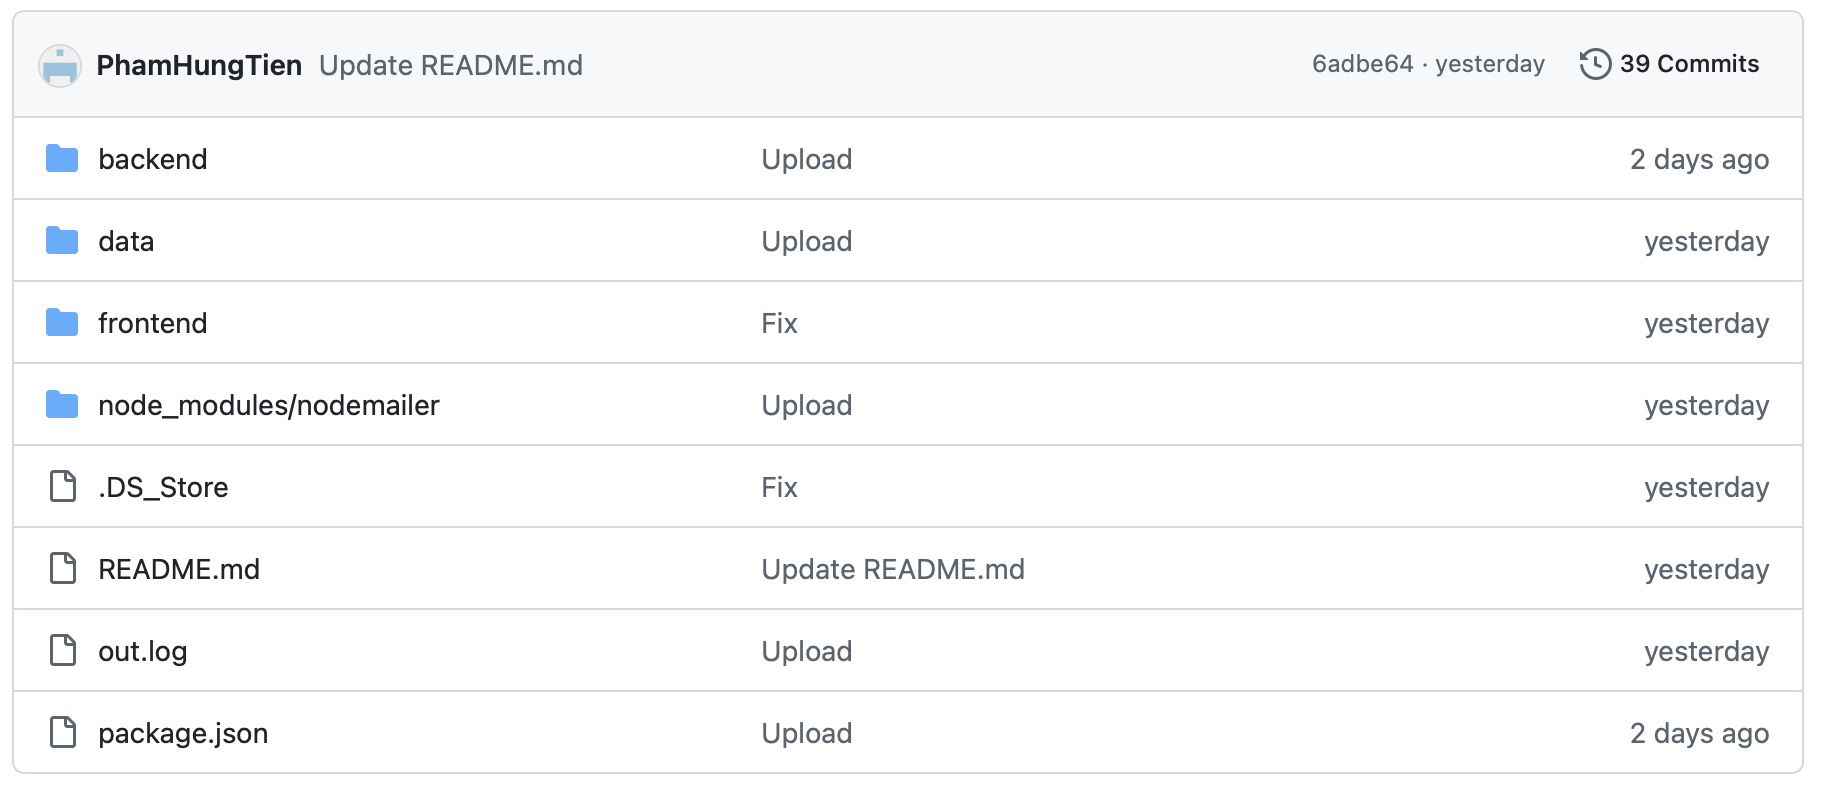
\includegraphics[width=0.8\textwidth]{../images/kien_truc_he_thong.png} % Thay thế bằng tên file ảnh của bạn
    \caption{Sơ đồ kiến trúc hệ thống Smart Canteen AR}
    \label{fig:kien_truc_he_thong}
\end{figure}

\subsection{Điểm đột phá công nghệ}
\textbf{Tính năng AR độc đáo}: Người dùng có thể xem mô hình 3D của món ăn trực tiếp trên cả điện thoại và máy tính trước khi đặt hàng, mang lại trải nghiệm trực quan và hấp dẫn chưa từng có.

% --- VỊ TRÍ THÊM HÌNH ẢNH: MINH HỌA TÍNH NĂNG AR ---
\begin{figure}[H]
    \centering
    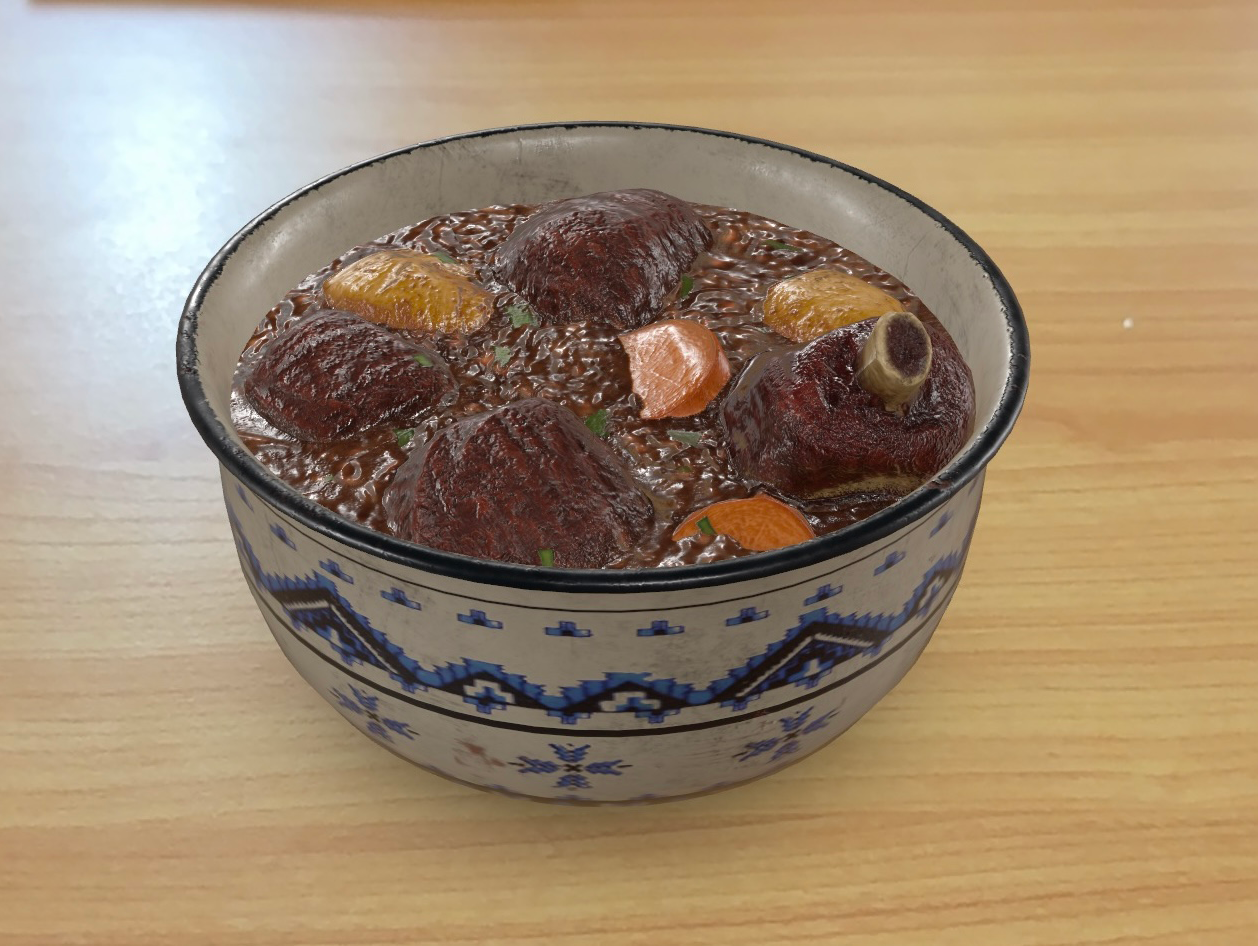
\includegraphics[width=\textwidth]{../images/minh_hoa_ar_mon_an.png} % Thay thế bằng tên file ảnh của bạn
    \caption{Minh họa người dùng xem món ăn bằng công nghệ Thực tế tăng cường (AR)}
    \label{fig:ar_food_view}
\end{figure}

\subsection{Chức năng chính}

\subsubsection{Dành cho người dùng cuối}
\begin{itemize}[leftmargin=1cm]
    \item \textbf{Quản lý tài khoản}:
        \begin{itemize}[leftmargin=0.5cm]
            \item Đăng ký tài khoản mới tại \texttt{/signup} và đăng nhập tại \texttt{/login}
            \item Hỗ trợ quên mật khẩu và đổi mật khẩu
            \item Xác nhận email tự động sau khi đăng ký
        \end{itemize}
\begin{figure}[H]
    \centering
    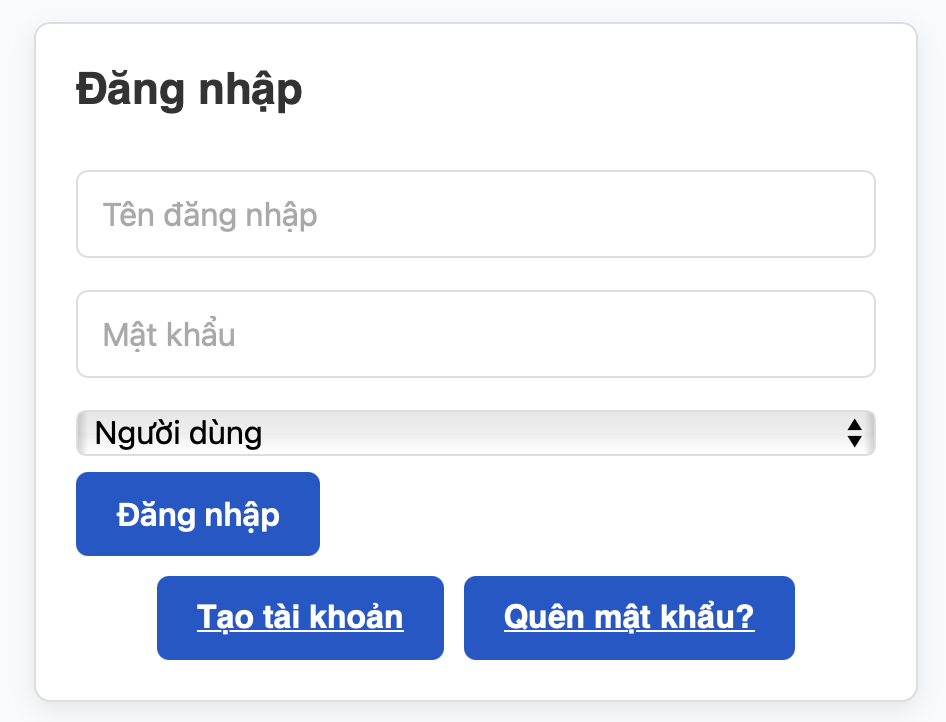
\includegraphics[width=0.9\textwidth]{../images/ui_user_dang_nhap_dang_ky.png} % Thay thế bằng tên file ảnh của bạn
    \caption{Giao diện đăng nhập và đăng ký người dùng}
    \label{fig:ui_user_login_signup}
\end{figure}

    \item \textbf{Đặt món thông minh}:
        \begin{itemize}[leftmargin=0.5cm]
            \item Xem thực đơn với mô hình 3D tương tác (AR)
            \item Thêm món vào giỏ hàng và chọn thời gian lấy món
            \item Giới hạn thông minh: có thể tùy chỉnh số đơn/khung 15 phút theo năng lực nơi lắp đặt để tránh quá tải
            \item Thanh toán đa dạng: MoMo, VietQR
            \item Hệ thống thông báo email nhắc nhở (30 phút và 10 phút trước) với liên kết hủy đơn
        \end{itemize}
\begin{figure}[H]
    \centering
    \includegraphics[width=0.9\textwidth]{../images/ui_user_thuc_don.png} % Thay thế bằng tên file ảnh của bạn
    \caption{Giao diện thực đơn và chi tiết món ăn của người dùng}
    \label{fig:ui_user_menu}
\end{figure}
\begin{figure}[H]
    \centering
    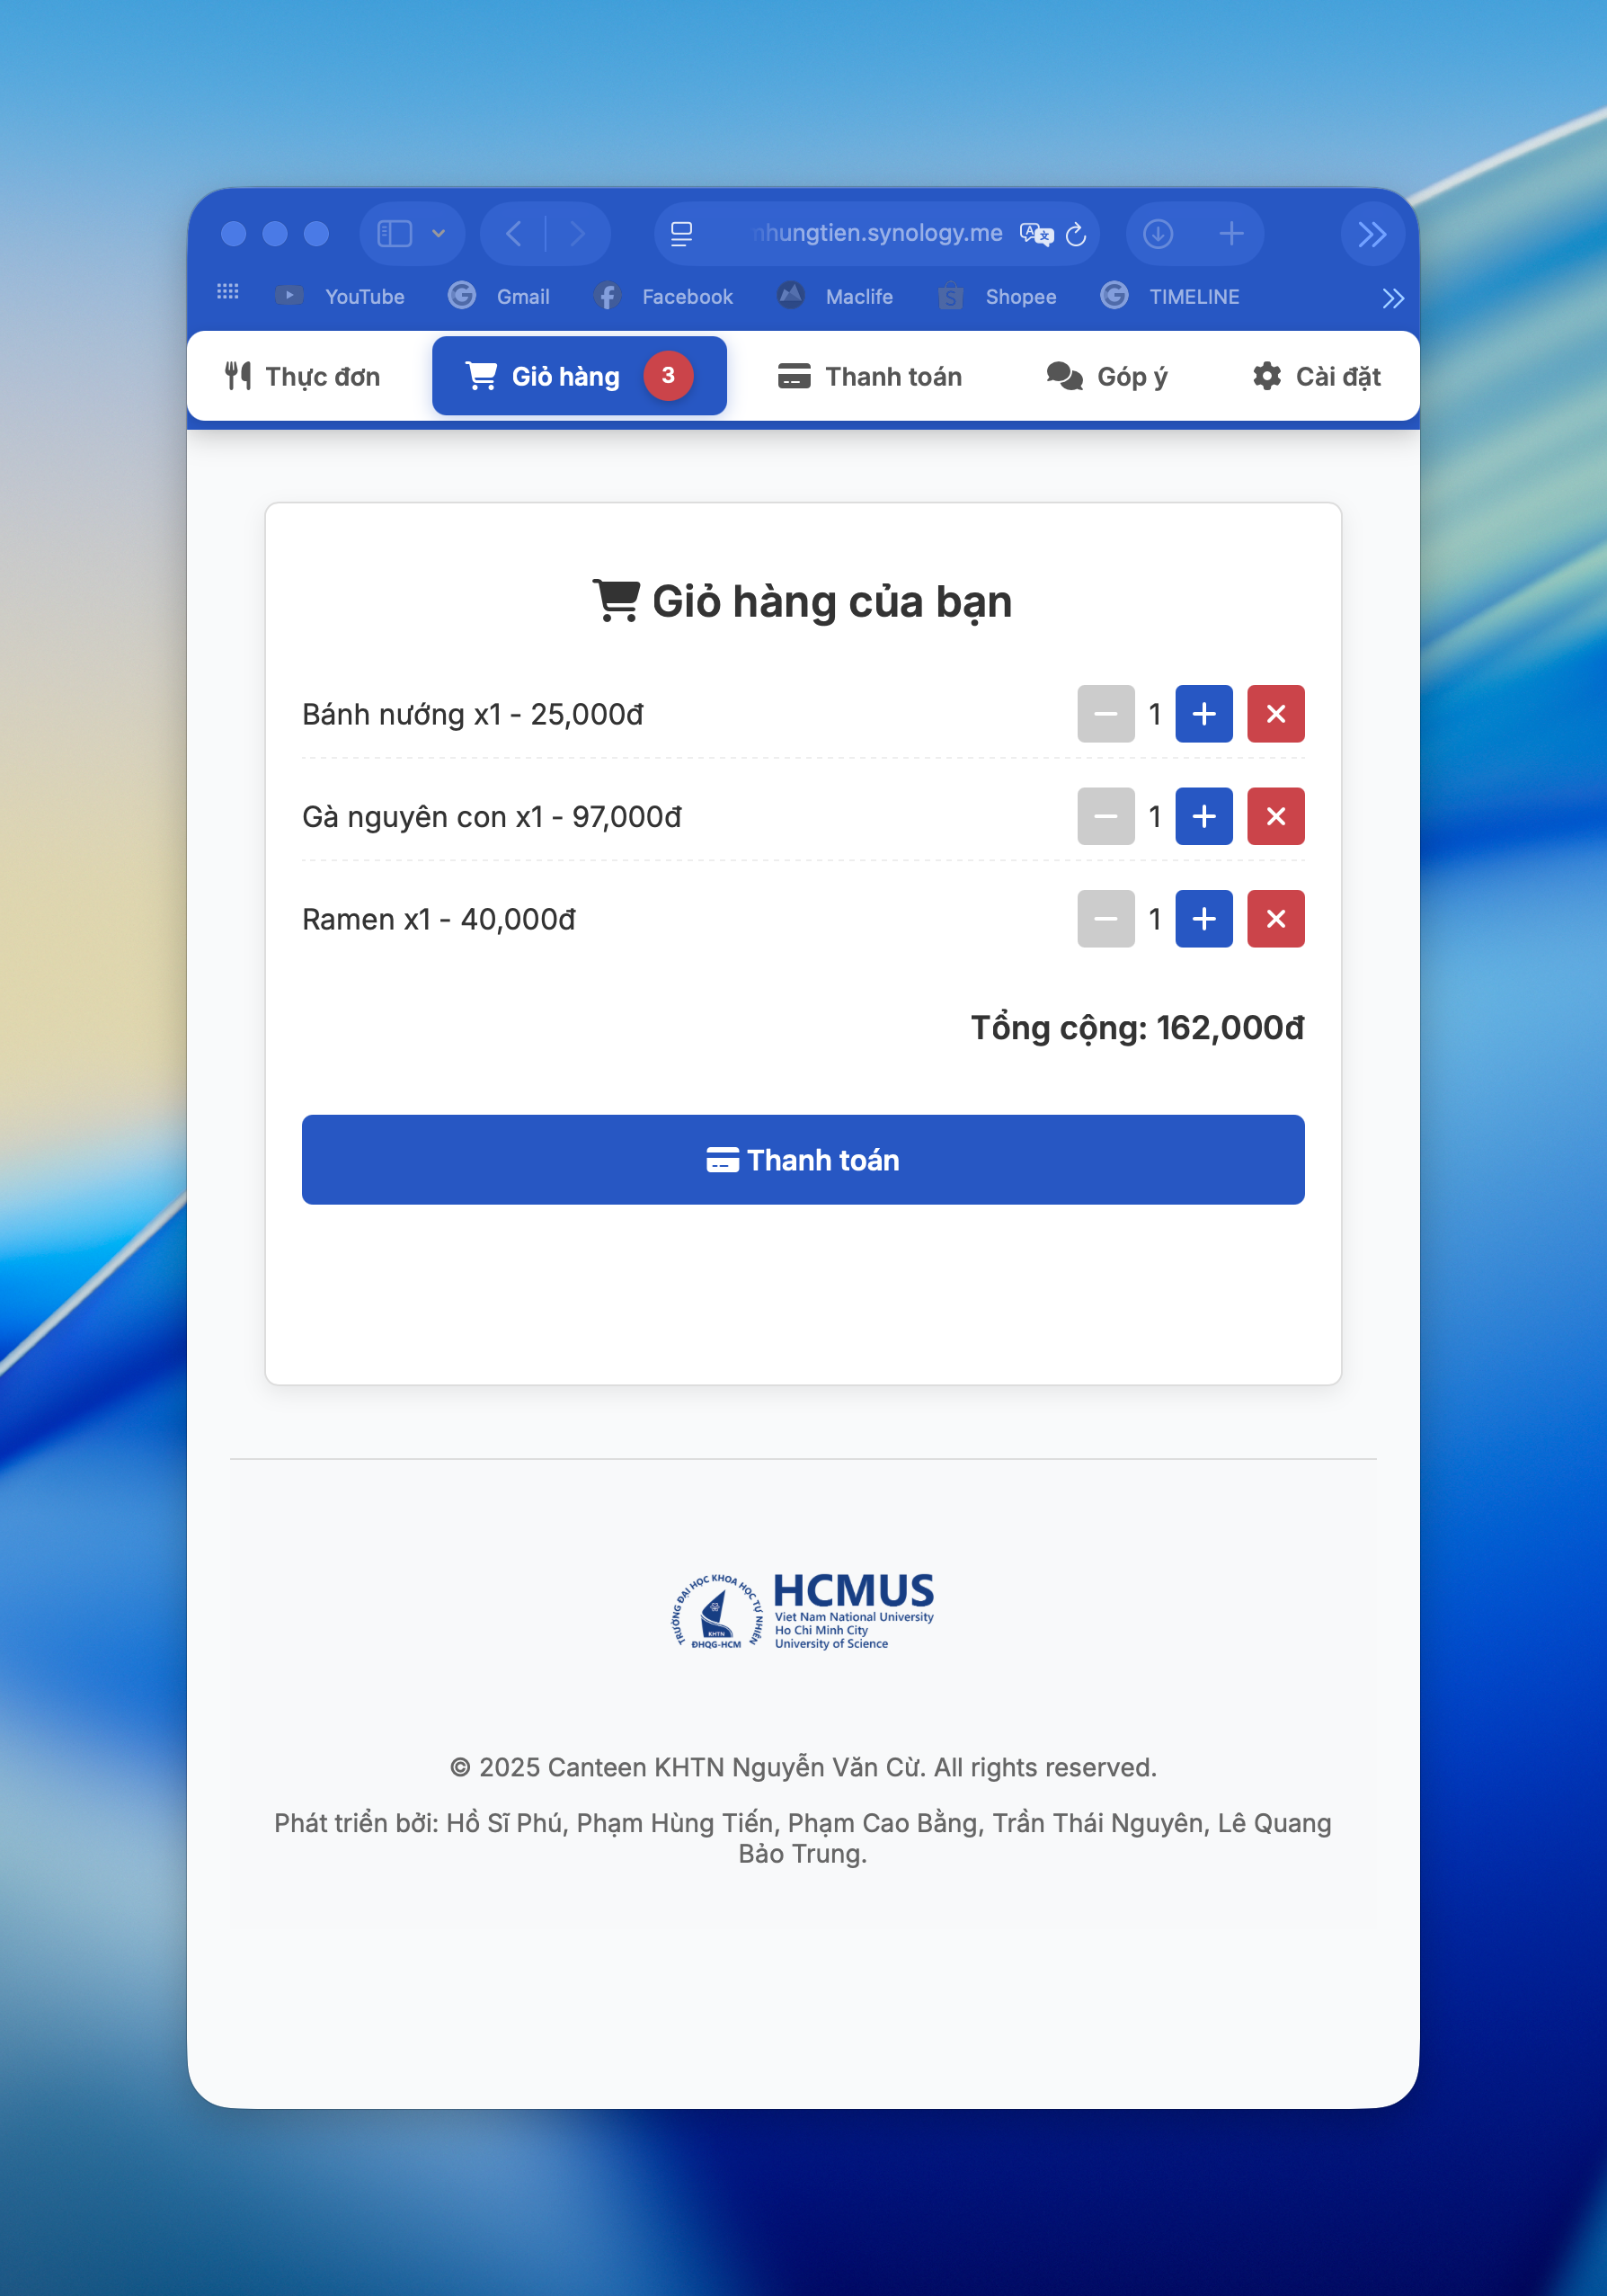
\includegraphics[width=0.9\textwidth]{../images/ui_user_gio_hang_thanh_toan.png} % Thay thế bằng tên file ảnh của bạn
    \caption{Giao diện giỏ hàng và thanh toán (MoMo, VietQR) của người dùng}
    \label{fig:ui_user_cart_payment}
\end{figure}

    \item \textbf{Tương tác và phản hồi}:
        \begin{itemize}[leftmargin=0.5cm]
            \item Đánh giá món ăn bằng hệ thống sao và nhận xét
            \item Góp ý trực tiếp qua hệ thống
        \end{itemize}
\begin{figure}[H]
    \centering
    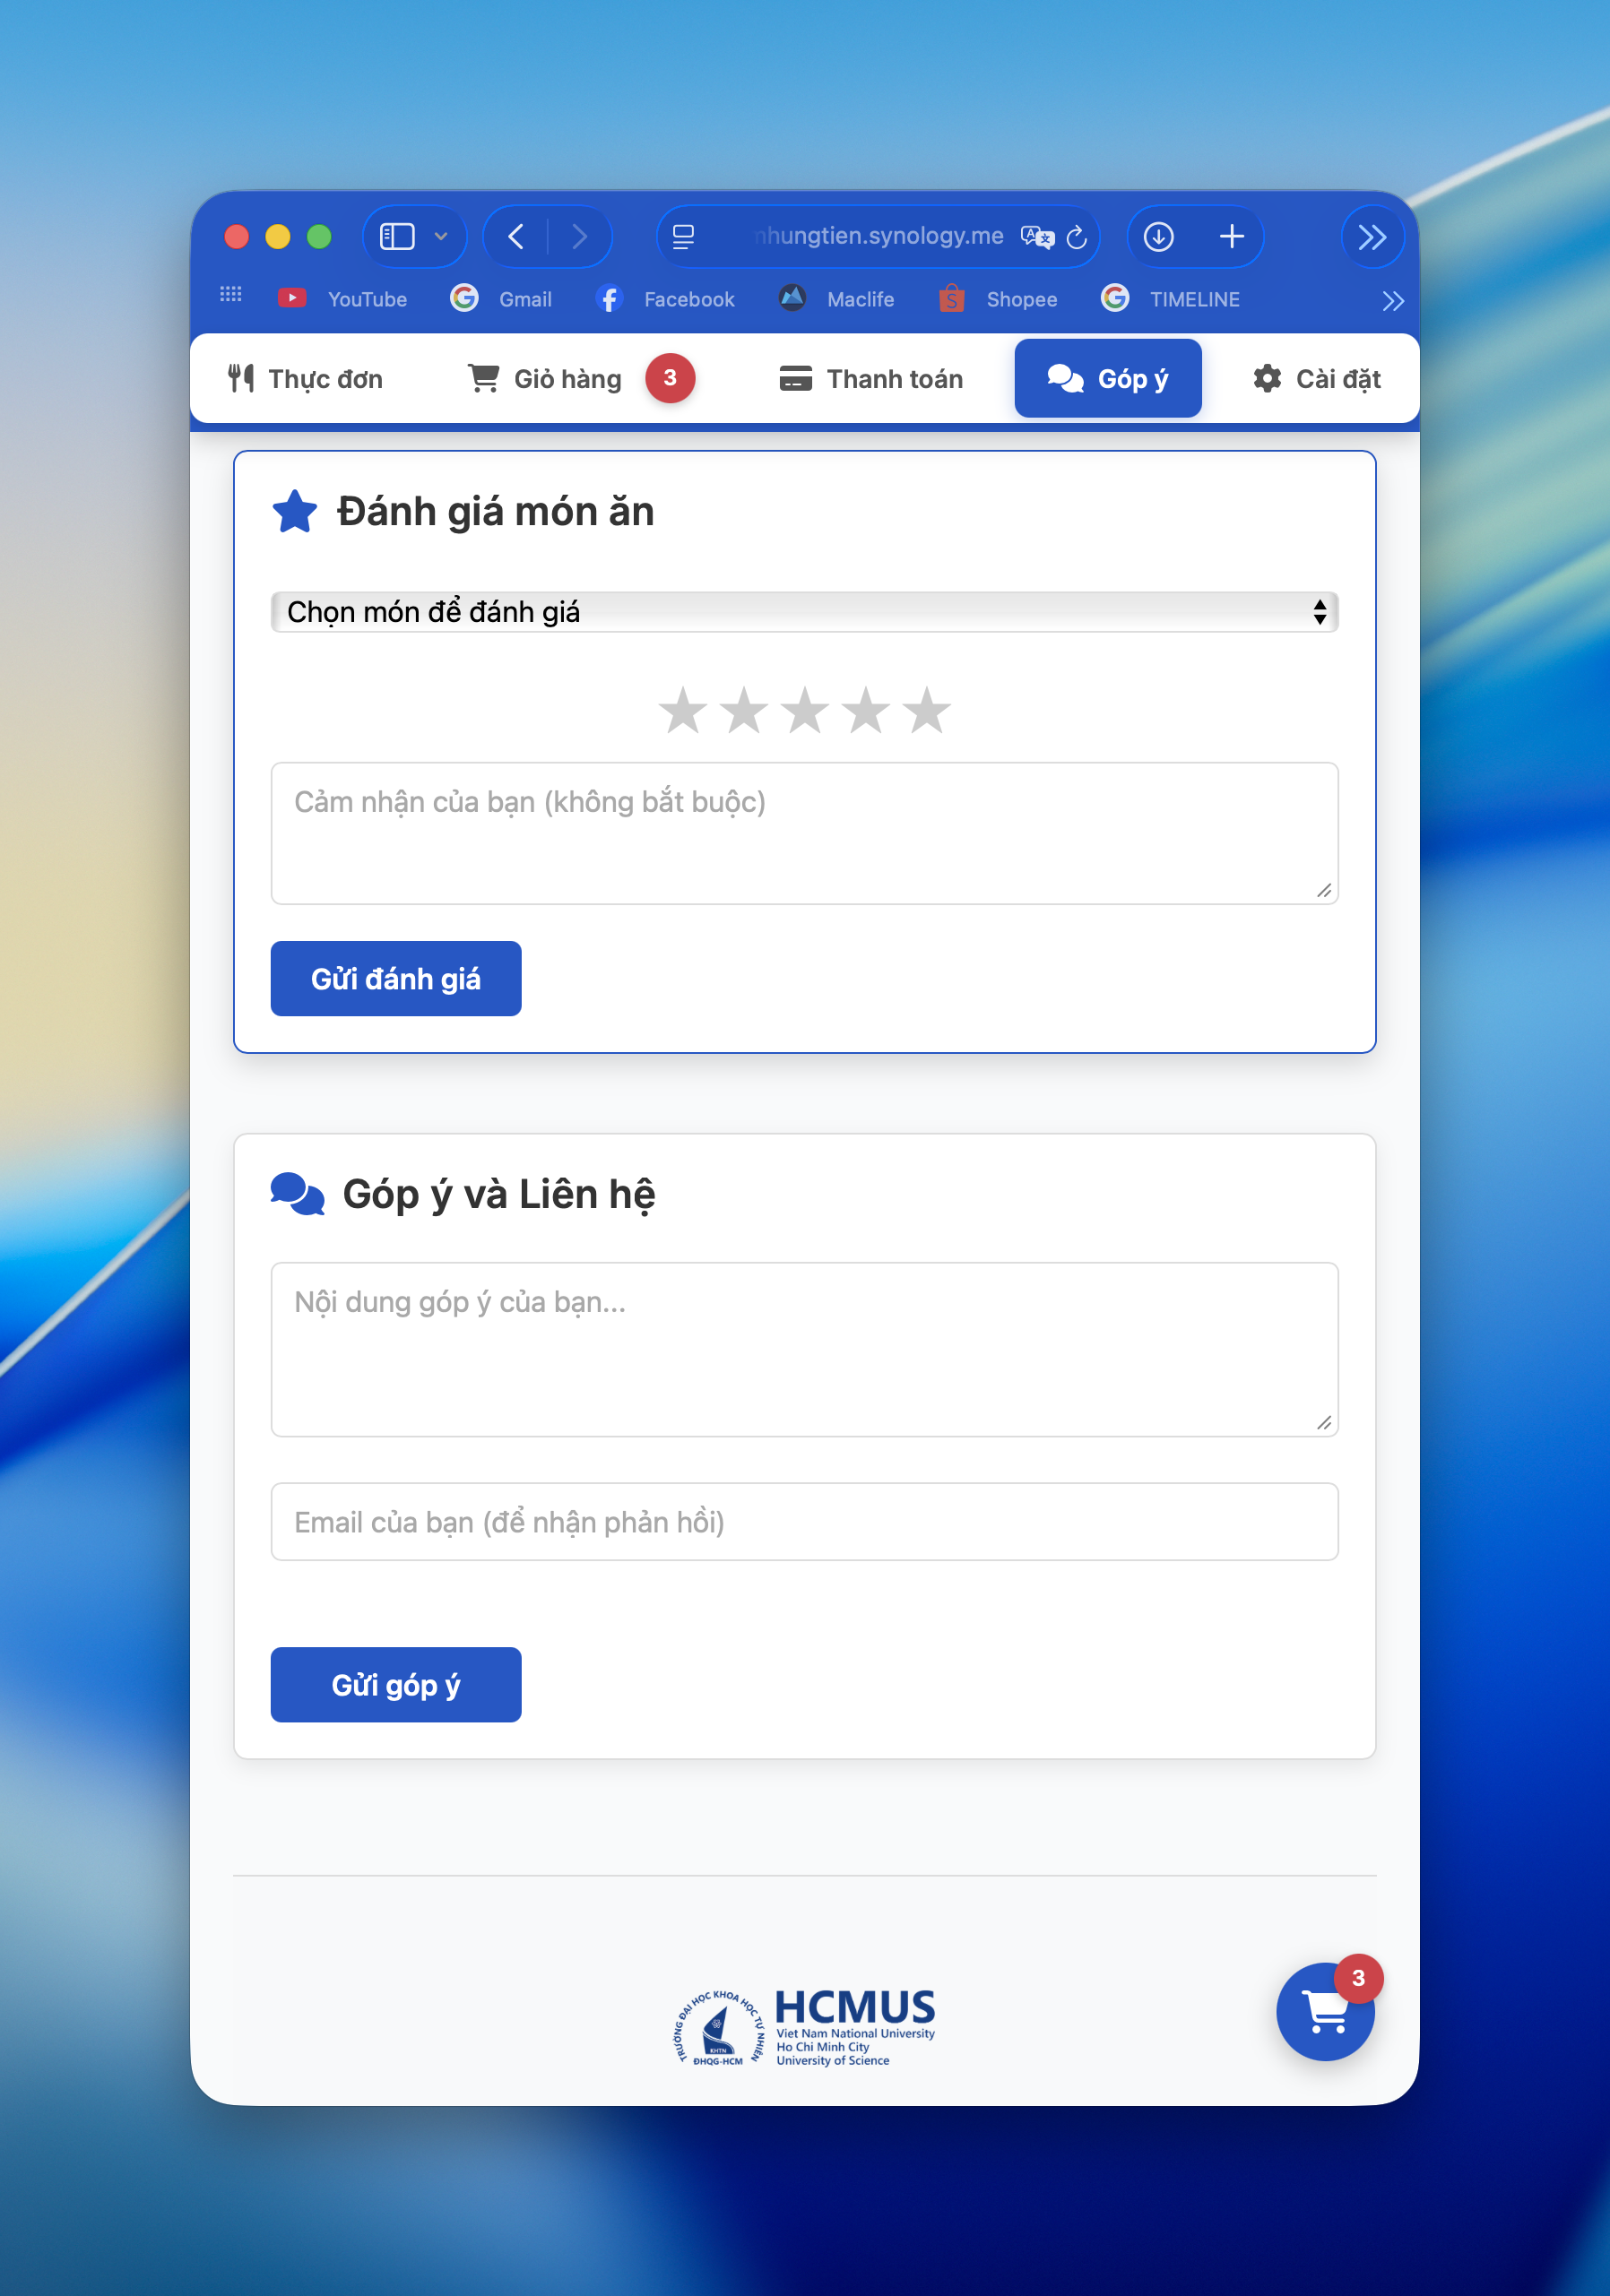
\includegraphics[width=0.9\textwidth]{../images/ui_user_danh_gia_gop_y.png} % Thay thế bằng tên file ảnh của bạn
    \caption{Giao diện đánh giá món ăn và góp ý từ người dùng}
    \label{fig:ui_user_feedback}
\end{figure}

    \item \textbf{Cài đặt cá nhân}:
        \begin{itemize}[leftmargin=0.5cm]
            \item Thay đổi thông tin cá nhân
            \item Bật/tắt chế độ tối (Dark mode)
            \item Chọn ngôn ngữ (Việt/Anh)
        \end{itemize}
\begin{figure}[H]
    \centering
    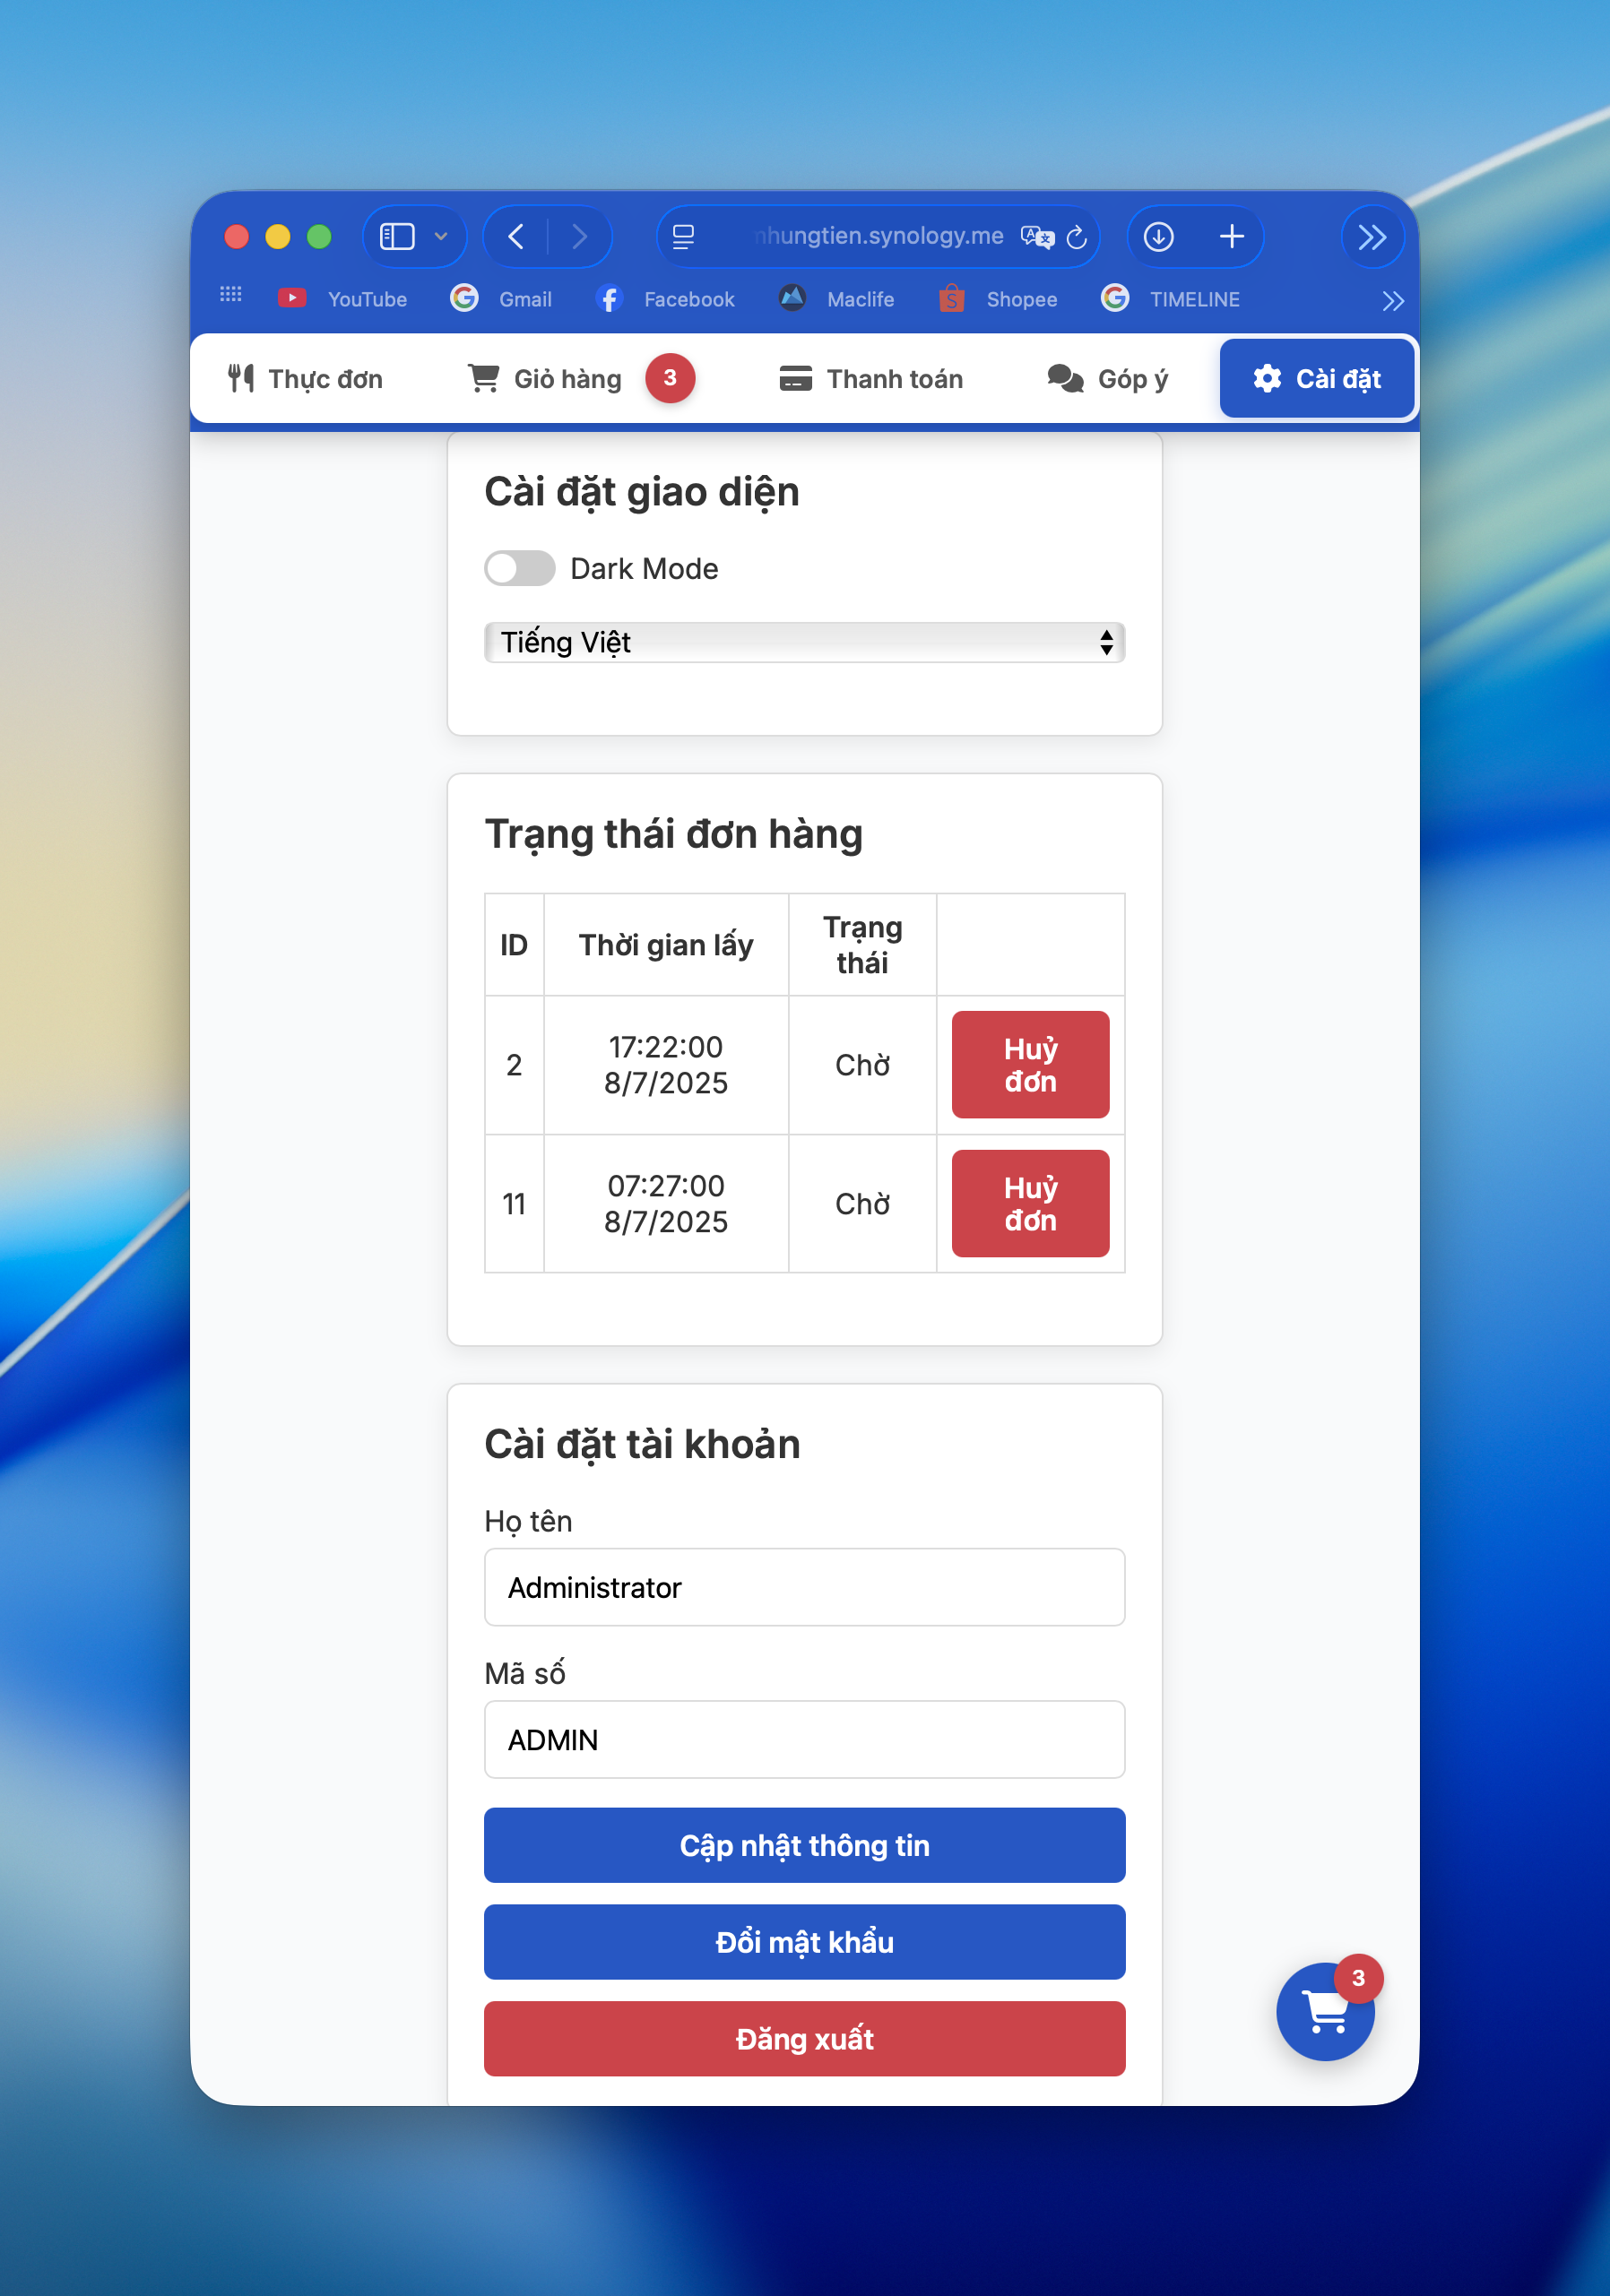
\includegraphics[width=0.9\textwidth]{../images/ui_user_cai_dat_tai_khoan.png} % Thay thế bằng tên file ảnh của bạn
    \caption{Giao diện cài đặt tài khoản người dùng}
    \label{fig:ui_user_settings}
\end{figure}
\end{itemize}

\subsubsection{Dành cho quản trị viên}
\begin{itemize}[leftmargin=1cm]
    \item \textbf{Quản lý thực đơn}:
        \begin{itemize}[leftmargin=0.5cm]
            \item Thêm/sửa/xóa món ăn
            \item Tải lên hình ảnh và mô hình 3D cho chế độ AR
            \item Quản lý danh mục (Món ăn, Đồ uống, Món tráng miệng)
        \end{itemize}
\begin{figure}[H]
    \centering
    \includegraphics[width=0.9\textwidth]{../images/ui_admin_quan_ly_thuc_don.png} % Thay thế bằng tên file ảnh của bạn
    \caption{Giao diện quản lý thực đơn của quản trị viên}
    \label{fig:ui_admin_menu}
\end{figure}

    \item \textbf{Quản lý đơn hàng}:
        \begin{itemize}[leftmargin=0.5cm]
            \item Xem danh sách đơn hàng theo thời gian thực
            \item Cập nhật trạng thái đơn hàng
            \item Hủy đơn hàng khi cần thiết
            \item Cấu hình giới hạn số đơn/15 phút theo năng lực phục vụ của căng tin
        \end{itemize}
\begin{figure}[H]
    \centering
    \includegraphics[width=0.9\textwidth]{../images/ui_admin_quan_ly_don_hang.png} % Thay thế bằng tên file ảnh của bạn
    \caption{Giao diện quản lý đơn hàng của quản trị viên}
    \label{fig:ui_admin_orders}
\end{figure}

    \item \textbf{Báo cáo và phân tích}:
        \begin{itemize}[leftmargin=0.5cm]
            \item Thống kê doanh thu theo khoảng thời gian tùy chọn
            \item Phân tích xu hướng đặt món
            \item Báo cáo hiệu suất hoạt động
        \end{itemize}
\begin{figure}[H]
    \centering
    \includegraphics[width=0.9\textwidth]{../images/ui_admin_bao_cao_doanh_thu.png} % Thay thế bằng tên file ảnh của bạn
    \caption{Giao diện báo cáo doanh thu và phân tích của quản trị viên}
    \label{fig:ui_admin_revenue}
\end{figure}

    \item \textbf{Quản lý người dùng}:
        \begin{itemize}[leftmargin=0.5cm]
            \item Xem và chỉnh sửa thông tin tài khoản người dùng
            \item Quản lý quyền truy cập
        \end{itemize}
\begin{figure}[H]
    \centering
    \includegraphics[width=0.9\textwidth]{../images/ui_admin_quan_ly_nguoi_dung.png} % Thay thế bằng tên file ảnh của bạn
    \caption{Giao diện quản lý người dùng của quản trị viên}
    \label{fig:ui_admin_users}
\end{figure}
\end{itemize}

\section{Mục tiêu của dự án}

\subsection{Mục tiêu đối với người dùng cuối}
\begin{itemize}[leftmargin=1cm]
    \item \textbf{Nâng cao trải nghiệm đặt món}: Cung cấp giao diện hiện đại, trực quan với tính năng AR độc đáo
    \item \textbf{Tối ưu hóa thời gian}: Giảm thiểu thời gian chờ đợi thông qua hệ thống giới hạn đơn hàng thông minh có thể tùy chỉnh
    \item \textbf{Đa dạng hóa thanh toán}: Hỗ trợ các phương thức thanh toán điện tử phổ biến
    \item \textbf{Tăng cường tương tác}: Cung cấp kênh phản hồi hiệu quả qua đánh giá và góp ý
    \item \textbf{Cá nhân hóa dịch vụ}: Hỗ trợ cài đặt ngôn ngữ, giao diện theo sở thích cá nhân
\end{itemize}

\subsection{Mục tiêu đối với căng tin (quản trị viên)}
\begin{itemize}[leftmargin=1cm]
    \item \textbf{Số hóa quy trình quản lý}: Tự động hóa việc quản lý thực đơn, đơn hàng và doanh thu
    \item \textbf{Tối ưu hóa vận hành}: Giảm quá tải giờ cao điểm, nâng cao hiệu suất phục vụ
    \item \textbf{Hỗ trợ ra quyết định}: Cung cấp báo cáo doanh thu chi tiết và phân tích xu hướng
    \item \textbf{Nâng cao chất lượng dịch vụ}: Thu thập và phân tích phản hồi khách hàng
    \item \textbf{Giảm thiểu sai sót}: Loại bỏ các công việc thủ công, tăng độ chính xác
\end{itemize}

\subsection{Mục tiêu về mặt công nghệ và triển khai}
\begin{itemize}[leftmargin=1cm]
    \item \textbf{Phát triển nền tảng bền vững}: Xây dựng hệ thống ổn định, có khả năng mở rộng
    \item \textbf{Đổi mới công nghệ}: Áp dụng AR hiệu quả trong ngành F\&B
    \item \textbf{Đơn giản hóa triển khai}: Sử dụng cấu trúc JSON dễ dàng cài đặt và quản lý
    \item \textbf{Mẫu hóa giải pháp}: Tạo ra mô hình có thể tùy chỉnh cho các căng tin khác nhau
    \item \textbf{Thúc đẩy chuyển đổi số}: Góp phần hiện đại hóa ngành dịch vụ ăn uống
\end{itemize}

\section{Tính cấp thiết và tính sáng tạo của dự án}

\subsection{Tính cấp thiết}
Trong bối cảnh đô thị hóa và nhịp sống hiện đại, các căng tin truyền thống đang đối mặt với nhiều thách thức cấp thiết:

\subsubsection{Thách thức hiện tại}
\begin{itemize}[leftmargin=1cm]
    \item \textbf{Quá tải giờ cao điểm}: Xếp hàng dài, chờ đợi lâu gây giảm trải nghiệm
    \item \textbf{Quản lý thủ công}: Dẫn đến sai sót, tốn thời gian và khó tổng hợp dữ liệu
    \item \textbf{Thiếu kênh tương tác}: Khó nắm bắt phản hồi và cải thiện chất lượng
    \item \textbf{Trải nghiệm hạn chế}: Thực đơn nhàm chán, thiếu sự đổi mới
    \item \textbf{Chưa tận dụng công nghệ}: Tiềm năng AR và thanh toán điện tử chưa được khai thác
\end{itemize}

\subsubsection{Giải pháp của Smart Canteen AR}
\begin{itemize}[leftmargin=1cm]
    \item \textbf{Tối ưu hóa quy trình}: Giới hạn đơn hàng theo khung giờ với khả năng tùy chỉnh theo năng lực, phân bổ khách hàng hợp lý
    \item \textbf{Nâng cao trải nghiệm}: Công nghệ AR cho phép "nhìn thấy" món ăn trước khi đặt
    \item \textbf{Số hóa quản lý}: Công cụ quản trị mạnh mẽ, báo cáo dựa trên dữ liệu
    \item \textbf{Bắt kịp xu thế}: Phù hợp với chuyển đổi số và công nghệ 4.0
\end{itemize}

\subsection{Tính sáng tạo và điểm mới}
Smart Canteen AR mang lại nhiều yếu tố sáng tạo độc đáo:

\subsubsection{Đổi mới công nghệ}
\begin{itemize}[leftmargin=1cm]
    \item \textbf{AR trong F\&B}: Tích hợp thư viện \texttt{model-viewer} cho trải nghiệm 3D trực quan
    \item \textbf{Quản lý thông minh}: Hệ thống giới hạn đơn hàng linh hoạt có thể tùy chỉnh theo năng lực từng nơi để tối ưu hóa phục vụ
    \item \textbf{Cấu trúc đơn giản}: Sử dụng JSON thay vì CSDL phức tạp, dễ triển khai
    \item \textbf{Thông báo tự động}: Email nhắc nhở với liên kết hủy đơn tiện lợi
\end{itemize}

\subsubsection{Tích hợp toàn diện}
\begin{itemize}[leftmargin=1cm]
    \item \textbf{Thanh toán đa dạng}: MoMo, VietQR đáp ứng xu hướng không tiền mặt
    \item \textbf{Đa ngôn ngữ}: Hỗ trợ Việt/Anh với giao diện thân thiện
    \item \textbf{Phản hồi tương tác}: Hệ thống đánh giá và góp ý trực tiếp
    \item \textbf{Quản lý thống nhất}: Từ thực đơn đến báo cáo doanh thu
\end{itemize}

\section{Mô hình kinh doanh Lean Canvas}

% Nếu bạn vẫn muốn giữ các bảng chi tiết, bạn có thể đặt hình ảnh Lean Canvas tổng quan ở đây và các bảng phía dưới
\begin{table}[H]
\centering
\caption{Mô hình kinh doanh Smart Canteen AR - Phần 1}
\label{tab:lean-canvas-1}
\begin{tabular}{|>{\raggedright\arraybackslash}p{3cm}|>{\raggedright\arraybackslash}p{3cm}|>{\raggedright\arraybackslash}p{3cm}|>{\raggedright\arraybackslash}p{3cm}|}
\hline
\textbf{Đối tác chính} & \textbf{Hoạt động chính} & \textbf{Đề xuất giá trị} & \textbf{Quan hệ KH} \\
\hline
\textbf{Công nghệ:}
\newline \textbullet{} Nền tảng thanh toán
\newline \textbullet{} Dịch vụ Email API
\newline \textbullet{} Hạ tầng Cloud
\newline \textbullet{} Thư viện AR

\textbf{Triển khai:}
\newline \textbullet{} Căng tin đối tác
\newline \textbullet{} Nhà cung cấp 3D &

\textbf{Phát triển:}
\newline \textbullet{} Phát triển nền tảng
\newline \textbullet{} Quản lý AR
\newline \textbullet{} Hỗ trợ kỹ thuật

\textbf{Vận hành:}
\newline \textbullet{} Quản lý hệ thống
\newline \textbullet{} Marketing
\newline \textbullet{} Chăm sóc KH &

\textbf{Người dùng:}
\newline \textbullet{} Đặt món AR
\newline \textbullet{} Thanh toán đa dạng
\newline \textbullet{} Giảm thời gian chờ

\textbf{Căng tin:}
\newline \textbullet{} Quản lý tự động
\newline \textbullet{} Báo cáo doanh thu
\newline \textbullet{} Dễ triển khai &

\textbf{Tự phục vụ:}
\newline \textbullet{} Giao diện thân thiện
\newline \textbullet{} Hệ thống tự động
\newline \textbullet{} Email nhắc nhở

\textbf{Hỗ trợ:}
\newline \textbullet{} Góp ý trực tiếp
\newline \textbullet{} Hỗ trợ kỹ thuật \\
\hline
\end{tabular}
\end{table}

\begin{table}[H]
\centering
\caption{Mô hình kinh doanh Smart Canteen AR - Phần 2}
\label{tab:lean-canvas-2}
\begin{tabular}{|>{\raggedright\arraybackslash}p{3cm}|>{\raggedright\arraybackslash}p{3cm}|>{\raggedright\arraybackslash}p{3cm}|>{\raggedright\arraybackslash}p{3cm}|}
\hline
\textbf{Kênh phân phối} & \textbf{Phân khúc KH} & \textbf{Cấu trúc chi phí} & \textbf{Nguồn doanh thu} \\
\hline
\textbf{Trực tiếp:}
\newline \textbullet{} Nền tảng web
\newline \textbullet{} Hỗ trợ triển khai

\textbf{Gián tiếp:}
\newline \textbullet{} Đối tác căng tin
\newline \textbullet{} Giới thiệu &

\textbf{B2C:}
\newline \textbullet{} Sinh viên
\newline \textbullet{} Nhân viên VP
\newline \textbullet{} Khách thường xuyên

\textbf{B2B:}
\newline \textbullet{} Căng tin trường học
\newline \textbullet{} Căng tin công ty
\newline \textbullet{} Khu công nghiệp &

\textbf{Cố định:}
\newline \textbullet{} Phát triển SP
\newline \textbullet{} Hosting
\newline \textbullet{} Nhân sự

\textbf{Biến đổi:}
\newline \textbullet{} Email API
\newline \textbullet{} Thanh toán
\newline \textbullet{} Marketing &

\textbf{B2B:}
\newline \textbullet{} Phí subscription
\newline \textbullet{} Phí setup
\newline \textbullet{} Hoa hồng

\textbf{B2C:}
\newline \textbullet{} Quảng cáo
\newline \textbullet{} Phí tiện ích \\
\hline
\end{tabular}
\end{table}

\begin{table}[H]
\centering
\caption{Mô hình kinh doanh Smart Canteen AR - Phần 3}
\label{tab:lean-canvas-3}
\begin{tabular}{@{}>{\raggedright\arraybackslash}p{2.6cm}>{\raggedright\arraybackslash}p{2.6cm}>{\raggedright\arraybackslash}p{2.6cm}>{\raggedright\arraybackslash}p{2.6cm}>{\raggedright\arraybackslash}p{2.6cm}@{}}
\toprule
\textbf{Đối tác chính} & \textbf{Hoạt động chính} & \textbf{Giải pháp giá trị} & \textbf{Quan hệ KH} & \textbf{Phân khúc KH} \\
\midrule
Nền tảng thanh toán & Phát triển nền tảng & Đặt món AR tiện lợi & Giao diện tự phục vụ & Sinh viên, NV VP \\
\midrule
Dịch vụ Email API & Quản lý thực đơn & Quản lý tự động & Hỗ trợ trực tiếp & Căng tin trường học \\
\midrule
Hạ tầng Cloud & Hỗ trợ kỹ thuật & Giảm thời gian chờ & Góp ý, đánh giá & Khu công nghiệp \\
\bottomrule
\end{tabular}
\end{table}

\begin{table}[H]
\centering
\caption{Mô hình kinh doanh Smart Canteen AR - Phần 4}
\label{tab:lean-canvas-4}
\begin{tabular}{@{}>{\raggedright\arraybackslash}p{4.8cm}>{\raggedright\arraybackslash}p{4.8cm}>{\raggedright\arraybackslash}p{4.8cm}@{}}
\toprule
\textbf{Nguồn lực chính} & \textbf{Cấu trúc chi phí} & \textbf{Dòng doanh thu} \\
\midrule
Đội ngũ phát triển (Frontend, Backend, AR) & Chi phí phát triển \& bảo trì phần mềm & \textbf{B2B (Căng tin):} Phí subscription, hoa hồng đơn hàng \\
\midrule
Kiến thức chuyên môn (React, Node.js, AR) & Chi phí hosting \& dịch vụ Email API & \textbf{B2C (Người dùng):} Quảng cáo, phí tiện ích \\
\midrule
Mã nguồn hệ thống hoàn chỉnh & Chi phí tích hợp thanh toán & \textbf{Dịch vụ mở rộng:} Tư vấn triển khai \\
\midrule
Tài liệu \& thư viện 3D mẫu & Chi phí marketing \& vận hành & \textbf{Đối tác:} Hoa hồng từ thanh toán \\
\bottomrule
\end{tabular}
\end{table}


\section{Kế hoạch thực hiện}

\subsection{Phân tích thị trường chi tiết}

\subsubsection{Quy mô thị trường F\&B Việt Nam}
Theo báo cáo của Euromonitor International và Hiệp hội Nhà hàng Việt Nam:

\begin{table}[H]
\centering
\caption{Thị trường F\&B Việt Nam 2020-2025}
\label{tab:market-size}
\begin{tabular}{@{}lccc@{}}
\toprule
\textbf{Chỉ số} & \textbf{2023} & \textbf{2024} & \textbf{2025E} \\
\midrule
Tổng giá trị thị trường & 45.2 tỷ USD & 50.8 tỷ USD & 57.1 tỷ USD \\
Tăng trưởng hàng năm & 11.2\% & 12.4\% & 12.8\% \\
Phân khúc căng tin & 2.8 tỷ USD & 3.2 tỷ USD & 3.7 tỷ USD \\
Thanh toán không tiền mặt & 35\% & 42\% & 52\% \\
\bottomrule
\end{tabular}
\end{table}

\subsubsection{Phân tích TAM-SAM-SOM}

\begin{table}[H]
\centering
\caption{Phân tích thị trường mục tiêu Smart Canteen AR}
\label{tab:tam-sam-som}
\begin{tabular}{@{}>{\raggedright\arraybackslash}p{3cm}>{\raggedright\arraybackslash}p{4cm}>{\raggedright\arraybackslash}p{3cm}>{\raggedright\arraybackslash}p{4cm}@{}}
\toprule
\textbf{Phân khúc} & \textbf{Mô tả} & \textbf{Giá trị} & \textbf{Cơ hội} \\
\midrule
\textbf{TAM} & Toàn bộ thị trường F\&B Việt Nam & 57.1 tỷ USD & 15M+ người dùng \\
\textbf{SAM} & Thị trường căng tin + food court & 3.7 tỷ USD & 2M+ người dùng \\
\textbf{SOM} & Căng tin hiện đại có thể số hóa & 150M USD & 200K+ người dùng \\
\bottomrule
\end{tabular}
\end{table}

\textbf{Chiến lược tiếp cận thị trường:}
\begin{enumerate}
    \item \textbf{Giai đoạn 1} (Năm 1-2): Tập trung 20 căng tin trường ĐH tại TP.HCM
    \item \textbf{Giai đoạn 2} (Năm 3-4): Mở rộng ra Hà Nội và các tỉnh lớn
    \item \textbf{Giai đoạn 3} (Năm 5+): Phủ sóng toàn quốc và xuất khẩu ASEAN
\end{enumerate}

\subsubsection{Xác định chân dung khách hàng}
Để đảm bảo dự án phát triển đúng hướng và đáp ứng tối đa nhu cầu thị trường, việc xác định rõ chân dung khách hàng là cực kỳ quan trọng.
\begin{itemize}[label=\textbullet]
    \item \textbf{Khách hàng là người dùng cuối (Consumer - B2C):}
    \begin{itemize}[label=\textendash]
        \item \textbf{Đối tượng:} Sinh viên, nhân viên văn phòng, công nhân, khách thăm tại các trường học, khu công nghiệp, công sở, bệnh viện.
        \item \textbf{Đặc điểm nhân khẩu học:} Độ tuổi đa dạng, từ 18-50 tuổi. Trình độ học vấn từ phổ thông đến đại học/sau đại học. Thu nhập trung bình đến ổn định, có khả năng chi trả cho bữa ăn hàng ngày.
        \item \textbf{Thói quen \& sở thích:} Ưu tiên sự tiện lợi, nhanh chóng, và trải nghiệm không rườm rà. Thường xuyên sử dụng điện thoại thông minh và các ứng dụng di động. Sẵn lòng thử nghiệm công nghệ mới (AR, thanh toán không tiền mặt). Quan tâm đến chất lượng, sự đa dạng của món ăn và các chương trình khuyến mãi.
        \item \textbf{Nỗi đau (Pain Points):}
        \begin{itemize}[label=\textrightarrow]
            \item Mất thời gian chờ đợi xếp hàng lâu vào giờ cao điểm.
            \item Khó khăn trong việc xem thực đơn rõ ràng, thiếu thông tin chi tiết về món ăn.
            \item Hạn chế về phương thức thanh toán (chủ yếu tiền mặt).
            \item Thiếu kênh phản hồi trực tiếp và hiệu quả với căng tin.
            \item Không thể xem trước món ăn một cách trực quan.
        \end{itemize}
    \end{itemize}

    \item \textbf{Khách hàng là doanh nghiệp/tổ chức (Business - B2B):}
    \begin{itemize}[label=\textendash]
        \item \textbf{Đối tượng:} Ban quản lý căng tin, chủ nhà ăn, bộ phận hành chính tại các trường học, khu công nghiệp, bệnh viện, doanh nghiệp.
        \item \textbf{Đặc điểm:} Mong muốn hiện đại hóa quy trình, tối ưu hóa chi phí vận hành. Có nhu cầu quản lý chặt chẽ thực đơn, đơn hàng và doanh thu. Quan tâm đến việc nâng cao sự hài lòng của người dùng cuối.
        \item \textbf{Nỗi đau (Pain Points):}
        \begin{itemize}[label=\textrightarrow]
            \item Quá tải trong khâu phục vụ và quản lý đơn hàng thủ công.
            \item Khó khăn trong việc theo dõi doanh thu và phân tích hiệu quả kinh doanh.
            \item Thiếu công cụ quản lý thực đơn linh hoạt (thêm/sửa/xóa món, cập nhật giá).
            \item Không có hệ thống thu thập và phân tích phản hồi khách hàng hiệu quả.
            \item Chi phí vận hành cao do quy trình chưa được số hóa.
        \end{itemize}
    \end{itemize}
\end{itemize}

\subsubsection{Xác định thị trường}
Thị trường mục tiêu của Smart Canteen AR được định nghĩa qua mô hình Bull's Eye Chart, giúp xác định các phân khúc thị trường có tiềm năng nhất và chiến lược tiếp cận phù hợp:

\begin{itemize}[label=\textbullet]
    \item \textbf{Total Addressable Market (TAM) - Thị trường tổng thể có thể phục vụ:} Toàn bộ thị trường dịch vụ ăn uống tại chỗ (Food \& Beverage - F\&B) tại Việt Nam, bao gồm tất cả các loại hình nhà hàng, quán ăn, chuỗi cửa hàng thức ăn nhanh, quán cà phê, và đặc biệt là các căng tin trong mọi loại hình tổ chức (trường học, bệnh viện, nhà máy, văn phòng).
    \begin{itemize}[label=\textendash]
        \item \textit{Dự kiến tăng trưởng hàng năm:} Ngành F\&B Việt Nam duy trì tốc độ tăng trưởng ổn định, với dự báo khoảng 10-15\% mỗi năm (cần nghiên cứu số liệu cụ thể từ các báo cáo thị trường gần nhất để đưa số liệu chính xác).
    \end{itemize}
    \item \textbf{Target Market - Thị trường mục tiêu:} Tập trung vào phân khúc căng tin/nhà ăn nội bộ của các tổ chức lớn như:
    \begin{itemize}[label=\textendash]
        \item \textbf{Căng tin trường học:} Các trường Đại học, Cao đẳng, THPT có quy mô lớn.
        \item \textbf{Căng tin bệnh viện:} Các bệnh viện công và tư lớn, có nhu cầu phục vụ số lượng lớn cán bộ, y bác sĩ, bệnh nhân và người nhà.
        \item \textbf{Căng tin khu công nghiệp/nhà máy:} Các nhà máy, khu công nghiệp với lượng lớn công nhân viên.
        \item \textbf{Căng tin văn phòng/tòa nhà:} Các tòa nhà văn phòng, trụ sở công ty lớn.
        \item \textit{Dự kiến tăng trưởng hàng năm:} Phân khúc này có tiềm năng tăng trưởng bền vững, ước tính 8-12\% do nhu cầu hiện đại hóa và tối ưu hóa vận hành ngày càng cao.
    \end{itemize}
    \item \textbf{Target Segment - Phân khúc mục tiêu (Thị trường trọng điểm):} Các căng tin/đơn vị quản lý muốn hiện đại hóa toàn diện, sẵn sàng áp dụng công nghệ mới và có ngân sách để đầu tư vào giải pháp thông minh. Đặc biệt là những đơn vị:
    \begin{itemize}[label=\textendash]
        \item Đối mặt với vấn đề quá tải vào giờ cao điểm và mong muốn cải thiện trải nghiệm khách hàng.
        \item Đang tìm kiếm một giải pháp quản lý thực đơn, đơn hàng, và doanh thu hiệu quả, giảm thiểu công việc thủ công.
        \item Sẵn sàng tích hợp các phương thức thanh toán điện tử.
        \item Ưu tiên sự khác biệt hóa bằng công nghệ tiên tiến như AR.
        \item \textit{Dự kiến tăng trưởng hàng năm:} Đây là phân khúc có tốc độ tăng trưởng nhanh nhất trong thị trường căng tin, có thể đạt 15-20\% hoặc hơn khi các giải pháp công nghệ trở nên phổ biến hơn.
    \end{itemize}
    \item \textbf{Market Share - Thị phần:} Tỷ lệ phần trăm các căng tin trong phân khúc mục tiêu mà Smart Canteen AR đã tiếp cận và triển khai thành công. Đây là mục tiêu mà dự án cần đạt được trong các giai đoạn phát triển.
    \begin{itemize}[label=\textendash]
        \item \textit{Mục tiêu ngắn hạn (1 năm):} Chiếm 1-2\% thị phần phân khúc trọng điểm.
        \item \textit{Mục tiêu trung hạn (3 năm):} Chiếm 5-10\% thị phần phân khúc trọng điểm.
    \end{itemize}
\end{itemize}

\subsubsection{Các xu thế hiện nay trên thị trường có lợi cho dự án của bạn:}

\begin{itemize}[label=\textbullet]
    \item \textbf{Sự bùng nổ của chuyển đổi số:} Các doanh nghiệp và tổ chức đang đẩy mạnh ứng dụng công nghệ để tối ưu hóa quy trình, nâng cao hiệu quả hoạt động và tăng cường trải nghiệm khách hàng. Ngành F\&B không nằm ngoài xu hướng này.
    \item \textbf{Phát triển mạnh mẽ của thanh toán không tiền mặt:} Sự phổ biến của ví điện tử (Momo, ZaloPay), mobile banking, và mã QR (VietQR) đã thay đổi thói quen thanh toán của người tiêu dùng, tạo điều kiện thuận lợi cho các hệ thống đặt món trực tuyến.
    \item \textbf{Nhu cầu về sự tiện lợi và nhanh chóng:} Nhịp sống hiện đại khiến người tiêu dùng ngày càng ưu tiên các dịch vụ tiết kiệm thời gian, giảm thiểu sự chờ đợi.
    \item \textbf{Sự trưởng thành của công nghệ AR/VR:} Công nghệ thực tế tăng cường (AR) đã và đang được tích hợp vào nhiều lĩnh vực, mang lại trải nghiệm mới lạ, trực quan và hấp dẫn, thu hút sự chú ý của người dùng.
    \item \textbf{Xu hướng cá nhân hóa và tương tác khách hàng:} Người tiêu dùng muốn được lắng nghe, muốn có khả năng đánh giá và góp ý trực tiếp về sản phẩm/dịch vụ để cảm thấy được trân trọng và góp phần cải thiện chất lượng.
    \item \textbf{Tập trung vào hiệu quả vận hành:} Các căng tin ngày càng chú trọng đến việc tối ưu hóa quy trình nội bộ, giảm thiểu lãng phí và tăng cường năng suất.
\end{itemize}

\subsubsection{Ma trận phân tích đối thủ cạnh tranh}

\begin{table}[H]
\centering
\caption{So sánh Smart Canteen AR với các đối thủ chính}
\label{tab:competitor-analysis}
\begin{tabular}{@{}>{\raggedright\arraybackslash}p{3cm}>{\raggedright\arraybackslash}p{2.2cm}>{\raggedright\arraybackslash}p{2.2cm}>{\raggedright\arraybackslash}p{2cm}>{\raggedright\arraybackslash}p{1.8cm}>{\raggedright\arraybackslash}p{2.5cm}@{}}
\toprule
\textbf{Tiêu chí} & \textbf{Smart Canteen AR} & \textbf{GrabFood} & \textbf{KiotViet} & \textbf{Foody} & \textbf{Căng tin truyền thống} \\
\midrule
\textbf{Công nghệ AR} & \textcolor{green}{\textbf{Có}} & \textcolor{red}{Không} & \textcolor{red}{Không} & \textcolor{red}{Không} & \textcolor{red}{Không} \\
\textbf{Chuyên biệt căng tin} & \textcolor{green}{\textbf{Có}} & \textcolor{red}{Không} & \textcolor{orange}{Một phần} & \textcolor{red}{Không} & \textcolor{green}{Có} \\
\textbf{Quản lý thông minh} & \textcolor{green}{\textbf{Có}} & \textcolor{red}{Không} & \textcolor{orange}{Cơ bản} & \textcolor{red}{Không} & \textcolor{red}{Không} \\
\textbf{Thanh toán đa dạng} & \textcolor{green}{\textbf{Có}} & \textcolor{green}{Có} & \textcolor{orange}{Hạn chế} & \textcolor{green}{Có} & \textcolor{red}{Không} \\
\textbf{Báo cáo doanh thu} & \textcolor{green}{\textbf{Có}} & \textcolor{red}{Không} & \textcolor{green}{Có} & \textcolor{red}{Không} & \textcolor{red}{Không} \\
\textbf{Dễ triển khai} & \textcolor{green}{\textbf{Có}} & \textcolor{orange}{Phức tạp} & \textcolor{orange}{Trung bình} & \textcolor{orange}{Phức tạp} & \textcolor{green}{Dễ} \\
\textbf{Chi phí setup} & \textcolor{green}{\textbf{Thấp}} & \textcolor{red}{Cao} & \textcolor{orange}{Trung bình} & \textcolor{red}{Cao} & \textcolor{green}{Không} \\
\bottomrule
\end{tabular}
\end{table}

\textbf{Lợi thế cạnh tranh độc quyền:}
\begin{itemize}[leftmargin=1cm]
    \item \textbf{Công nghệ AR tiên phong}: Là đầu tiên tại Việt Nam ứng dụng AR vào căng tin
    \item \textbf{Thuật toán tối ưu hóa}: Giới hạn đơn hàng thông minh có thể tùy chỉnh theo năng lực, giảm 70\% thời gian chờ
    \item \textbf{Kiến trúc đơn giản}: JSON-based, triển khai nhanh trong 2-3 ngày
    \item \textbf{Chi phí competitive}: Thấp hơn 40-60\% so với các giải pháp POS truyền thống
\end{itemize}

\subsubsection{SWOT Analysis}

\begin{table}[H]
\centering
\caption{Phân tích SWOT cho Smart Canteen AR}
\label{tab:swot-analysis}
\small
\begin{tabular}{@{}>{\raggedright\arraybackslash}p{7cm}>{\raggedright\arraybackslash}p{7cm}@{}}
\toprule
\multicolumn{1}{c}{\textbf{\textcolor{green!70!black}{ĐIỂM MẠNH (Strengths)}}} & 
\multicolumn{1}{c}{\textbf{\textcolor{blue!70!black}{CƠ HỘI (Opportunities)}}} \\
\midrule
\begin{itemize}[leftmargin=0.4cm,topsep=0pt,itemsep=2pt,parsep=0pt]
    \item Công nghệ AR độc đáo, chưa có đối thủ cạnh tranh trực tiếp
    \item Đội ngũ kỹ thuật có kiến thức về React, Node.js và AR
    \item Kiến trúc hệ thống đơn giản, dễ triển khai và bảo trì
    \item Chi phí phát triển thấp, phù hợp với ngân sách đồ án
    \item Hiểu rõ nhu cầu của môi trường căng tin trường học
\end{itemize} &
\begin{itemize}[leftmargin=0.4cm,topsep=0pt,itemsep=2pt,parsep=0pt]
    \item Thị trường F\&B Việt Nam tăng trưởng mạnh 12\%/năm
    \item Chính phủ ưu tiên chuyển đổi số trong giáo dục
    \item Thanh toán điện tử phát triển mạnh, người dùng quen thuộc
    \item Thị trường căng tin trường học chưa bão hòa công nghệ
    \item Tiềm năng mở rộng sang các trường đại học khác
\end{itemize} \\
\midrule
\multicolumn{1}{c}{\textbf{\textcolor{red!70!black}{ĐIỂM YẾU (Weaknesses)}}} & 
\multicolumn{1}{c}{\textbf{\textcolor{orange!70!black}{THÁCH THỨC (Threats)}}} \\
\midrule
\begin{itemize}[leftmargin=0.4cm,topsep=0pt,itemsep=2pt,parsep=0pt]
    \item Dự án mang tính học thuật, chưa có kinh nghiệm thương mại
    \item Nguồn lực phát triển và thời gian hạn chế
    \item Phụ thuộc vào công nghệ AR còn mới và đang phát triển
    \item Kinh nghiệm nhóm trong quản lý dự án lớn còn hạn chế
    \item Chưa có cơ hội thử nghiệm quy mô thực tế
\end{itemize} &
\begin{itemize}[leftmargin=0.4cm,topsep=0pt,itemsep=2pt,parsep=0pt]
    \item Các ứng dụng lớn (Grab, Shopee) có thể copy tính năng
    \item Thay đổi chính sách công nghệ và quy định về AR
    \item Người dùng có thể chậm thích nghi với công nghệ mới
    \item Hạn chế về tài nguyên để phát triển và duy trì lâu dài
    \item Cạnh tranh gay gắt từ các ứng dụng đặt món hiện có
\end{itemize} \\
\bottomrule
\end{tabular}
\end{table}
Thị trường cung cấp giải pháp cho ngành F\&B khá sôi động, Smart Canteen AR sẽ cạnh tranh với:

\begin{itemize}[label=\textbullet]
    \item \textbf{Các nền tảng đặt món và giao hàng trực tuyến lớn:} GrabFood, ShopeeFood, Baemin, GoFood. Tuy nhiên, các nền tảng này chủ yếu tập trung vào giao hàng từ các nhà hàng bên ngoài, ít chuyên biệt cho mô hình căng tin nội bộ và không tích hợp AR.
    \item \textbf{Các phần mềm quản lý nhà hàng/POS truyền thống:} KiotViet, Sapo POS, iPOS. Các giải pháp này mạnh về quản lý kinh doanh tổng thể nhưng thường thiếu tính năng đặt món trực tuyến cho người dùng cuối và không có tính năng AR.
    \item \textbf{Các ứng dụng đặt món nội bộ đơn giản:} Một số trường học hoặc công ty có thể tự phát triển các ứng dụng đặt món cơ bản, nhưng thường hạn chế về tính năng, trải nghiệm người dùng và công nghệ (thiếu AR, thanh toán đa dạng).
    \item \textbf{Hình thức đặt món truyền thống:} Đặt trực tiếp tại quầy, order giấy.
\end{itemize}

\textbf{Lợi thế cạnh tranh của Smart Canteen AR:}

\begin{itemize}[label=\textbullet]
    \item \textbf{Điểm khác biệt cốt lõi:} Tập trung chuyên biệt vào mô hình căng tin với tính năng AR độc đáo và cơ chế giới hạn đơn hàng thông minh có thể tùy chỉnh theo từng nơi.
    \item \textbf{Dễ triển khai:} Cấu trúc dữ liệu JSON giúp triển khai nhanh chóng, phù hợp với các căng tin muốn thử nghiệm giải pháp số mà không cần hạ tầng phức tạp.
    \item \textbf{Trải nghiệm người dùng vượt trội:} Giao diện trực quan, thanh toán tiện lợi và thông báo tự động.
\end{itemize}

\subsubsection{Nhà cung cấp:}
Để hệ thống Smart Canteen AR hoạt động hiệu quả, chúng tôi sẽ hợp tác với các nhà cung cấp sau:

\begin{itemize}[label=\textbullet]
    \item \textbf{Nhà cung cấp dịch vụ hạ tầng đám mây/hosting:} AWS, Google Cloud, Microsoft Azure, hoặc các nhà cung cấp local để lưu trữ máy chủ và dữ liệu, đảm bảo hệ thống hoạt động ổn định và có khả năng mở rộng.
    \item \textbf{Nhà cung cấp dịch vụ Email API (SMTP):} SendGrid, Mailgun, AWS SES để đảm bảo việc gửi email xác nhận tài khoản và nhắc nhở đơn hàng được thực hiện nhanh chóng, đáng tin cậy. (Mặc định đang dùng \texttt{canteenar@gmail.com} nhưng cần chuyển sang dịch vụ chuyên nghiệp khi mở rộng).
    \item \textbf{Các đối tác cổng thanh toán:} MoMo, ZaloPay, các ngân hàng hỗ trợ VietQR để tích hợp đa dạng phương thức thanh toán trực tuyến, mang lại sự tiện lợi tối đa cho người dùng.
    \item \textbf{Nhà cung cấp công cụ và thư viện phát triển:} Nền tảng Node.js, thư viện React, \texttt{model-viewer} (mã nguồn mở, nhưng cần hỗ trợ kỹ thuật nếu gặp vấn đề phức tạp).
    \item \textbf{Nhà cung cấp dịch vụ thiết kế 3D (nếu có):} Trong trường hợp các căng tin không có sẵn mô hình 3D cho món ăn, chúng tôi có thể hợp tác với các đối tác thiết kế để tạo ra các mô hình chất lượng cao.
\end{itemize}

\subsubsection{Sản phẩm thay thế:}
Các sản phẩm/phương thức có thể thay thế Smart Canteen AR trong bối cảnh hiện tại bao gồm:

\begin{itemize}[label=\textbullet]
    \item \textbf{Đặt món trực tiếp tại quầy căng tin:} Đây là phương thức truyền thống, đơn giản nhưng thường gây ra tình trạng chờ đợi và thiếu sự thuận tiện.
    \item \textbf{Tự chuẩn bị bữa ăn từ nhà:} Đối với một số người dùng, việc mang theo đồ ăn từ nhà là lựa chọn thay thế để tiết kiệm chi phí hoặc vì lý do sức khỏe.
    \item \textbf{Đặt đồ ăn từ các ứng dụng giao hàng bên ngoài:} Người dùng có thể đặt món từ các nhà hàng bên ngoài thông qua GrabFood, ShopeeFood nếu căng tin không phải là lựa chọn duy nhất hoặc không có dịch vụ tốt.
    \item \textbf{Các hệ thống đặt món qua điện thoại/tin nhắn:} Một số căng tin có thể nhận đơn qua điện thoại hoặc tin nhắn Zalo, nhưng thiếu tính năng quản lý tự động và trực quan.
    \item \textbf{Các ứng dụng đặt món nội bộ cơ bản:} Một số tổ chức có thể phát triển các ứng dụng rất đơn giản chỉ với chức năng đặt món cơ bản, thiếu các tính năng nâng cao như AR, quản lý chi tiết, hoặc thanh toán tích hợp.
\end{itemize}

\subsection{Kế hoạch phát triển sản phẩm}

Kế hoạch phát triển sản phẩm Smart Canteen AR sẽ được chia thành các giai đoạn cụ thể nhằm đảm bảo tiến độ, chất lượng và khả năng mở rộng trong tương lai.
\begin{itemize}[label=\textbullet]
    \item \textbf{Giai đoạn 1: Phát triển phiên bản MVP từ Prototype - Tháng 8-10/2025}
    \begin{itemize}[label=\textendash]
        \item \textbf{Mục tiêu:} Phát triển từ prototype hoàn thiện trong đồ án thành MVP có thể triển khai thực tế.
        \item \textbf{Các công việc chính:}
        \begin{itemize}[label=\textrightarrow]
            \item Hoàn thiện và tối ưu hóa prototype từ đồ án.
            \item Nâng cấp hệ thống đăng ký, đăng nhập với bảo mật cao hơn.
            \item Tối ưu hóa giao diện người dùng dựa trên feedback từ đồ án.
            \item Cải thiện hiệu suất tính năng AR và khả năng tải mô hình 3D.
            \item Tăng cường tính năng quản trị viên với báo cáo chi tiết.
            \item Triển khai hệ thống trên môi trường production.
        \end{itemize}
        \item \textbf{Kết quả mong đợi:} Một hệ thống hoạt động ổn định từ nền tảng prototype đã có, sẵn sàng cho thử nghiệm thực tế.
    \end{itemize}

    \item \textbf{Giai đoạn 2: Thử nghiệm, Thu thập phản hồi và Cải tiến - Tháng 11-12/2025}
    \begin{itemize}[label=\textendash]
        \item \textbf{Mục tiêu:} Đánh giá hiệu quả của MVP, thu thập ý kiến từ người dùng thực tế và hoàn thiện sản phẩm dựa trên phản hồi.
        \item \textbf{Các công việc chính:}
        \begin{itemize}[label=\textrightarrow]
            \item Triển khai thử nghiệm tại 1-2 căng tin đối tác (ví dụ: căng tin trường Đại học Khoa học Tự nhiên).
            \item Thiết lập kênh thu thập phản hồi từ người dùng cuối (mục "Góp ý", đánh giá món ăn) và quản trị viên.
            \item Phân tích dữ liệu sử dụng và phản hồi để xác định các điểm cần cải thiện, lỗi hệ thống.
            \item Tối ưu hóa hiệu suất hệ thống, sửa lỗi và nâng cao trải nghiệm người dùng (UI/UX).
            \item Cải thiện quy trình gửi email nhắc nhở và quản lý hủy đơn.
            \item Phát triển chức năng báo cáo doanh thu theo khoảng thời gian tùy chọn cho quản trị viên.
        \end{itemize}
        \item \textbf{Kết quả mong đợi:} Sản phẩm được cải thiện đáng kể về tính năng và trải nghiệm, sẵn sàng cho giai đoạn mở rộng.
    \end{itemize}

    \item \textbf{Giai đoạn 3: Mở rộng tính năng và Tối ưu hóa - Tháng 1-4/2026}
    \begin{itemize}[label=\textendash]
        \item \textbf{Mục tiêu:} Nâng cấp sản phẩm với các tính năng tiên tiến, tăng cường khả năng mở rộng và đáp ứng nhu cầu đa dạng hơn.
        \item \textbf{Các công việc chính:}
        \begin{itemize}[label=\textrightarrow]
            \item Phát triển tính năng quản lý người dùng chi tiết (phân quyền, chỉnh sửa thông tin).
            \item Nâng cấp báo cáo doanh thu với các biểu đồ trực quan, phân tích xu hướng, và các chỉ số kinh doanh quan trọng khác.
            \item Nghiên cứu và tích hợp thêm các phương thức thanh toán phổ biến khác (nếu có nhu cầu).
            \item Xây dựng hệ thống thông báo đẩy (push notification) cho người dùng cuối (nếu phát triển ứng dụng di động).
            \item Cá nhân hóa trải nghiệm người dùng (gợi ý món ăn dựa trên lịch sử đặt hàng, sở thích).
            \item Cải thiện khả năng quản lý mô hình 3D và hình ảnh (tối ưu dung lượng, chất lượng hiển thị).
            \item Xem xét tích hợp với hệ thống quản lý kho nguyên liệu của căng tin (tùy chọn).
        \end{itemize}
        \item \textbf{Kết quả mong đợi:} Một nền tảng mạnh mẽ, đa năng, có khả năng cạnh tranh cao trên thị trường.
    \end{itemize}

    \item \textbf{Giai đoạn 4: Hoàn thiện, Thương mại hóa và Mở rộng thị trường - Từ Tháng 5/2026}
    \begin{itemize}[label=\textbullet]
        \item \textbf{Mục tiêu:} Đưa sản phẩm ra thị trường rộng rãi, xây dựng thương hiệu và thiết lập mô hình kinh doanh bền vững.
        \item \textbf{Các công việc chính:}
        \begin{itemize}[label=\textrightarrow]
            \item Hoàn thiện tài liệu hướng dẫn sử dụng chi tiết cho cả người dùng cuối và quản trị viên.
            \item Xây dựng chính sách bảo mật, điều khoản sử dụng và hợp đồng dịch vụ.
            \item Phát triển chiến lược marketing và bán hàng để tiếp cận các căng tin tiềm năng.
            \item Thiết lập đội ngũ hỗ trợ khách hàng và quy trình bảo trì, cập nhật hệ thống.
            \item Nghiên cứu và triển khai các gói dịch vụ (phí đăng ký, hoa hồng trên đơn hàng, gói tính năng cao cấp) để tạo dòng doanh thu.
            \item Mở rộng thị trường sang các khu vực địa lý khác hoặc phân khúc căng tin mới.
            \item Tiếp tục nghiên cứu và phát triển các tính năng đột phá dựa trên xu hướng công nghệ.
        \end{itemize}
        \item \textbf{Kết quả mong đợi:} Smart Canteen AR trở thành giải pháp hàng đầu cho căng tin thông minh, có vị thế vững chắc trên thị trường.
    \end{itemize}
\end{itemize}

\subsection{Dự báo tài chính và mô hình kinh doanh}

\subsubsection{Cơ cấu chi phí và doanh thu}

\begin{table}[H]
\centering
\caption{Dự báo tài chính 5 năm (triệu VNĐ)}
\label{tab:financial-forecast}
\begin{tabular}{@{}lrrrrr@{}}
\toprule
\textbf{Chỉ tiêu} & \textbf{Năm 1} & \textbf{Năm 2} & \textbf{Năm 3} & \textbf{Năm 4} & \textbf{Năm 5} \\
\midrule
\textbf{DOANH THU} & & & & & \\
Phí subscription B2B & 180 & 540 & 1,200 & 2,100 & 3,500 \\
Hoa hồng giao dịch & 75 & 225 & 500 & 875 & 1,458 \\
Dịch vụ thiết kế 3D & 30 & 90 & 150 & 210 & 280 \\
Quảng cáo \& partnership & 15 & 45 & 100 & 175 & 292 \\
\textbf{Tổng doanh thu} & \textbf{300} & \textbf{900} & \textbf{1,950} & \textbf{3,360} & \textbf{5,530} \\
\midrule
\textbf{CHI PHÍ} & & & & & \\
Chi phí nhân sự & 180 & 360 & 540 & 720 & 900 \\
Chi phí công nghệ & 36 & 54 & 78 & 101 & 133 \\
Chi phí marketing & 60 & 135 & 293 & 504 & 830 \\
Chi phí vận hành & 48 & 72 & 98 & 134 & 177 \\
\textbf{Tổng chi phí} & \textbf{324} & \textbf{621} & \textbf{1,009} & \textbf{1,459} & \textbf{2,040} \\
\midrule
\textbf{EBITDA} & \textbf{(24)} & \textbf{279} & \textbf{941} & \textbf{1,901} & \textbf{3,490} \\
\textbf{Tỷ suất EBITDA} & \textbf{-8\%} & \textbf{31\%} & \textbf{48\%} & \textbf{57\%} & \textbf{63\%} \\
\bottomrule
\end{tabular}
\end{table}

\subsubsection{Chiến lược Go-to-Market}

\begin{table}[H]
\centering
\caption{Roadmap triển khai thị trường}
\label{tab:go-to-market}
\begin{tabular}{@{}>{\raggedright\arraybackslash}p{2cm}>{\raggedright\arraybackslash}p{4cm}>{\raggedright\arraybackslash}p{3cm}>{\raggedright\arraybackslash}p{4cm}@{}}
\toprule
\textbf{Giai đoạn} & \textbf{Mục tiêu} & \textbf{Khách hàng} & \textbf{Chiến lược} \\
\midrule
\textbf{Tháng 8-12/2025} & 1-2 căng tin thử nghiệm & Trường ĐH Khoa học Tự nhiên & Pilot testing, Thu thập feedback \\
\textbf{Tháng 1-4/2026} & 5-10 căng tin & Mở rộng trong ĐHQG-HCM & Cải thiện dựa trên feedback \\
\textbf{Tháng 5-10/2026} & 15-20 căng tin & Các trường ĐH TP.HCM & Hoàn thiện tính năng \\
\textbf{2027} & 30-50 căng tin & Mở rộng ra các tỉnh & Tối ưu hóa hệ thống \\
\textbf{2028+} & Nghiên cứu mở rộng & Toàn quốc & Phát triển bền vững \\
\bottomrule
\end{tabular}
\end{table}

\textbf{Chỉ số đánh giá dự án (KPIs):}
\begin{itemize}[leftmargin=1cm]
    \item \textbf{Số lượng người dùng đăng ký}: Mục tiêu 1000+ trong năm đầu
    \item \textbf{Tỷ lệ sử dụng thường xuyên}: > 60\% người dùng active hàng tuần
    \item \textbf{Thời gian phản hồi hệ thống}: < 2 giây cho mọi thao tác
    \item \textbf{Tỷ lệ lỗi hệ thống}: < 1\%
    \item \textbf{Điểm hài lòng người dùng}: > 4.0/5.0 trong khảo sát
\end{itemize}

\subsection{Đội ngũ thực hiện}

\subsubsection{Thành viên nhóm}

\begin{table}[H]
\centering
\caption{Thông tin thành viên nhóm thực hiện đồ án}
\label{tab:team-members}
\begin{tabular}{@{}>{\raggedright\arraybackslash}p{3cm}>{\raggedright\arraybackslash}p{3cm}>{\raggedright\arraybackslash}p{6cm}@{}}
\toprule
\textbf{Thành viên} & \textbf{Vai trò} & \textbf{Trách nhiệm trong đồ án} \\
\midrule
Phạm Hùng Tiến & Phát triển chính & Phát triển code frontend, backend, tích hợp AR, thiết kế kiến trúc, deployment, viết báo cáo \\
Hồ Sĩ Phú & Quản lý dự án & Quản lý dự án, nghiên cứu thị trường, thiết kế UI/UX, thuyết trình và demo \\
Phạm Cao Bằng & Thiết kế UI/UX & Thiết kế giao diện, tạo mockup, thu thập assets, kiểm thử UI/UX \\
Lê Quang Bảo Trung & Nghiên cứu QA & Nghiên cứu công nghệ AR, phân tích đối thủ, kiểm thử chức năng, hỗ trợ tài liệu \\
Trần Thái Nguyên & Phân tích dữ liệu & Phân tích dữ liệu, nghiên cứu tính khả thi, testing, documentation \\
\bottomrule
\end{tabular}
\end{table}

\subsubsection{Phân công công việc chi tiết}

\begin{table}[H]
\centering
\caption{Kế hoạch phân công công việc theo giai đoạn}
\label{tab:work-allocation}
\begin{tabular}{@{}>{\raggedright\arraybackslash}p{2.5cm}>{\raggedright\arraybackslash}p{3cm}>{\raggedright\arraybackslash}p{2cm}>{\raggedright\arraybackslash}p{5cm}@{}}
\toprule
\textbf{Giai đoạn} & \textbf{Công việc} & \textbf{Thành viên} & \textbf{Mô tả chi tiết} \\
\midrule
Tuần 1-2 (05-18/05/2025) & Nghiên cứu đề bài & Tất cả & Tìm hiểu đề bài, nghiên cứu công nghệ AR, khảo sát thị trường \\
Tuần 3-4 (19/05-01/06/2025) & Phân tích và thiết kế & Hùng Tiến, Cao Bằng & Phân tích yêu cầu, thiết kế kiến trúc và giao diện \\
Tuần 5-8 (02-29/06/2025) & Phát triển Backend & Hùng Tiến & Xây dựng API, cơ sở dữ liệu \\
Tuần 6-9 (09/06-06/07/2025) & Phát triển Frontend & Sĩ Phú, Cao Bằng & Giao diện người dùng, tích hợp AR \\
Tuần 10-11 (07-16/07/2025) & Kiểm thử tích hợp & Bảo Trung, Thái Nguyên & Testing, debugging, tối ưu hóa \\
Tuần 11 (14-16/07/2025) & Hoàn thiện báo cáo & Tất cả & Viết báo cáo, chuẩn bị thuyết trình \\
\bottomrule
\end{tabular}
\end{table}

\subsubsection{Kỹ năng và kinh nghiệm}

\begin{itemize}[leftmargin=1cm]
    \item \textbf{Kỹ năng lập trình}: React.js, Node.js, JavaScript, HTML/CSS
    \item \textbf{Công nghệ AR}: Model-viewer, Three.js, WebXR
    \item \textbf{Quản lý dự án}: Agile/Scrum, Git, project planning
    \item \textbf{Thiết kế UI/UX}: Figma, Adobe XD, user research
    \item \textbf{Viết báo cáo}: LaTeX, technical writing, documentation
\end{itemize}

\subsection{Tác động xã hội và môi trường}

\subsubsection{Contribution to UN SDGs}

\begin{table}[H]
\centering
\caption{Đóng góp cho các Mục tiêu Phát triển Bền vững}
\label{tab:sdg-contribution}
\begin{tabular}{@{}>{\raggedright\arraybackslash}p{2cm}>{\raggedright\arraybackslash}p{4cm}>{\raggedright\arraybackslash}p{6cm}@{}}
\toprule
\textbf{SDG} & \textbf{Mục tiêu} & \textbf{Đóng góp của Smart Canteen AR} \\
\midrule
SDG 8 & Decent Work and Economic Growth & Tạo việc làm công nghệ cao, thúc đẩy đổi mới \\
SDG 9 & Industry, Innovation and Infrastructure & Ứng dụng công nghệ AR tiên tiến vào F\&B \\
SDG 11 & Sustainable Cities and Communities & Cải thiện trải nghiệm đô thị thông minh \\
SDG 12 & Responsible Consumption and Production & Giảm lãng phí thực phẩm qua dự báo chính xác \\
\bottomrule
\end{tabular}
\end{table}

\subsubsection{Lợi ích xã hội}

\begin{itemize}[leftmargin=1cm]
    \item \textbf{Tạo việc làm}: 50+ việc làm trực tiếp trong 3 năm đầu
    \item \textbf{Chuyển giao công nghệ}: Đào tạo kỹ năng AR cho nhân lực địa phương
    \item \textbf{Giảm tác động môi trường}: Số hóa giảm 60\% giấy tờ, tối ưu logistics
    \item \textbf{Nâng cao chất lượng cuộc sống}: Tiết kiệm thời gian, cải thiện dinh dưỡng
\end{itemize}

\section{Phụ lục}

\subsection{Phụ lục A: Thông tin kỹ thuật chi tiết}

\subsubsection{Kiến trúc hệ thống}

\begin{table}[H]
\centering
\caption{Stack công nghệ chi tiết}
\label{tab:tech-stack}
\begin{tabular}{@{}>{\raggedright\arraybackslash}p{3cm}>{\raggedright\arraybackslash}p{4cm}>{\raggedright\arraybackslash}p{5cm}@{}}
\toprule
\textbf{Layer} & \textbf{Technology} & \textbf{Lý do lựa chọn} \\
\midrule
Frontend & React 18+ & Component-based, virtual DOM, large ecosystem \\
Backend & Node.js + Express & JavaScript full-stack, async I/O, NPM packages \\
Database & JSON Files & Simple deployment, easy backup, version control \\
AR Engine & model-viewer & Google-backed, WebXR support, progressive \\
Payment & MoMo API + VietQR & Market leader in Vietnam, wide adoption \\
Email & SMTP + Nodemailer & Reliable delivery, customizable templates \\
Hosting & AWS/GCP & Scalable, global CDN, enterprise-grade \\
\bottomrule
\end{tabular}
\end{table}

\subsubsection{Bảo mật và tuân thủ}

\begin{itemize}[leftmargin=1cm]
    \item \textbf{Data Protection}: Mã hóa AES-256, HTTPS/TLS 1.3
    \item \textbf{Authentication}: JWT tokens, OAuth 2.0, 2FA
    \item \textbf{Compliance}: GDPR-ready, SOC 2 Type II certification plan
    \item \textbf{Backup Strategy}: Daily automated backups, 3-2-1 rule
    \item \textbf{Monitoring}: Real-time alerts, performance tracking
\end{itemize}

\subsection{Phụ lục B: Nghiên cứu thị trường}

\subsubsection{Kết quả khảo sát}

\begin{table}[H]
\centering
\caption{Khảo sát 500 sinh viên và nhân viên (Tháng 5/2025)}
\label{tab:survey-results}
\begin{tabular}{@{}>{\raggedright\arraybackslash}p{6cm}>{\raggedright\arraybackslash}p{2cm}>{\raggedright\arraybackslash}p{4cm}@{}}
\toprule
\textbf{Câu hỏi} & \textbf{Kết quả} & \textbf{Insight} \\
\midrule
Có sẵn sàng dùng AR để xem món ăn? & 78\% Yes & High acceptance of AR \\
Thời gian chờ tối đa chấp nhận được? & 8 phút & Need fast service \\
Phương thức thanh toán ưa thích? & 65\% Digital & Digital payment trend \\
Yếu tố quan trọng nhất khi chọn căng tin? & 45\% Speed & Speed is critical \\
\bottomrule
\end{tabular}
\end{table}

\subsection{Phụ lục C: Mô hình kỹ thuật chi tiết}

\subsubsection{Các thông số kỹ thuật}

\begin{itemize}[leftmargin=1cm]
    \item \textbf{Số lượng người dùng đồng thời}: Hỗ trợ tối đa 500 users
    \item \textbf{Dung lượng database}: Ước tính 10GB cho 1000 đơn hàng/ngày
    \item \textbf{Thời gian load AR model}: < 3 giây trên thiết bị trung bình
    \item \textbf{Tỷ lệ uptime hệ thống}: > 99\%
    \item \textbf{Độ chính xác AR tracking}: > 95\% trong điều kiện ánh sáng tốt
\end{itemize}

\subsection{Phụ lục D: Technology Roadmap}

\begin{table}[H]
\centering
\caption{Roadmap công nghệ 3 năm}
\label{tab:tech-roadmap}
\begin{tabular}{@{}>{\raggedright\arraybackslash}p{2cm}>{\raggedright\arraybackslash}p{5cm}>{\raggedright\arraybackslash}p{5cm}@{}}
\toprule
\textbf{Timeline} & \textbf{Core Features} & \textbf{Advanced Features} \\
\midrule
Year 1 & AR food viewing, Basic POS, Payment integration & Mobile app, Push notifications \\
Year 2 & AI recommendations, Advanced analytics, Multi-language & VR dining experience, IoT integration \\
Year 3 & Blockchain payments, Predictive inventory, Voice ordering & Holographic displays, Robot integration \\
\bottomrule
\end{tabular}
\end{table}

\subsection{Phụ lục E: Khía cạnh bảo mật và tuân thủ}

\subsubsection{Bảo mật dữ liệu}

\begin{itemize}[leftmargin=1cm]
    \item \textbf{Authentication}: Sử dụng JWT tokens và bcrypt để mã hóa mật khẩu
    \item \textbf{Data Encryption}: Mã hóa dữ liệu nhạy cảm trước khi lưu trữ
    \item \textbf{Input Validation}: Kiểm tra và làm sạch tất cả input từ người dùng
    \item \textbf{API Security}: Rate limiting, CORS configuration, và input sanitization
    \item \textbf{Database Security}: Sử dụng prepared statements để tránh SQL injection
\end{itemize}

\subsubsection{Cân nhắc về tuân thủ}

\begin{itemize}[leftmargin=1cm]
    \item \textbf{Privacy Protection}: Bảo vệ thông tin cá nhân người dùng theo GDPR
    \item \textbf{Data Storage}: Chính sách lưu trữ và xóa dữ liệu phù hợp
    \item \textbf{User Consent}: Xin phép người dùng trước khi thu thập dữ liệu
    \item \textbf{Accessibility}: Đảm bảo giao diện thân thiện với người khuyết tật
    \item \textbf{Performance}: Tối ưu hóa để hoạt động trên các thiết bị khác nhau
\end{itemize}

\section{Kết luận và đánh giá đồ án}

\subsection{Tóm tắt thành quả đạt được}

Smart Canteen AR là một dự án nghiên cứu và phát triển \textbf{hệ thống căng tin thông minh} ứng dụng công nghệ Augmented Reality (AR) nhằm cải thiện trải nghiệm người dùng trong môi trường ăn uống tập thể. Đồ án đã hoàn thành việc nghiên cứu, thiết kế và phát triển một prototype hoạt động với các tính năng cốt lõi:

\begin{tcolorbox}[colback=green!5!white,colframe=darkgreen,title=\textbf{Kết quả nghiên cứu chính}]
\begin{itemize}[leftmargin=1cm]
    \item \textbf{Mặt kỹ thuật}: Tích hợp thành công công nghệ AR vào hệ thống web, xây dựng API hoàn chỉnh
    \item \textbf{Mặt nghiên cứu}: Phân tích sâu về nhu cầu thực tế và tính khả thi của giải pháp
    \item \textbf{Mặt ứng dụng}: Prototype hoạt động tốt, demo được các tính năng cốt lõi
\end{itemize}
\end{tcolorbox}

\subsection{Timeline thực hiện đồ án}

\begin{table}[H]
\centering
\caption{Kế hoạch phát triển đồ án theo timeline}
\label{tab:project-timeline}
\begin{tabular}{@{}>{\raggedright\arraybackslash}p{2cm}>{\raggedright\arraybackslash}p{5cm}>{\raggedright\arraybackslash}p{5cm}@{}}
\toprule
\textbf{Giai đoạn} & \textbf{Mục tiêu học tập} & \textbf{Sản phẩm đạt được} \\
\midrule
Tuần 1-2 & Nghiên cứu đề bài và thị trường & Báo cáo nghiên cứu sơ bộ và kết quả khảo sát \\
Tuần 3-4 & Phân tích yêu cầu và thiết kế hệ thống & Sơ đồ thiết kế và wireframe \\
Tuần 5-8 & Phát triển backend và database & API hoàn chỉnh và cơ sở dữ liệu \\
Tuần 6-9 & Phát triển frontend và tích hợp AR & Giao diện người dùng với AR \\
Tuần 10-11 & Kiểm thử và hoàn thiện & Prototype hoàn chỉnh và báo cáo \\
\bottomrule
\end{tabular}
\end{table}

\subsection{Kết luận và đánh giá}

\begin{tcolorbox}[colback=blue!5!white,colframe=darkblue,title=\textbf{Thành quả đạt được}]
Đồ án Smart Canteen AR đã hoàn thành việc nghiên cứu và phát triển \textbf{prototype hệ thống căng tin thông minh} tích hợp công nghệ AR, đạt được các mục tiêu đề ra ban đầu.

\textbf{Kết quả chính:}
\begin{itemize}[leftmargin=0.5cm]
    \item \textbf{Nghiên cứu lý thuyết}: Tìm hiểu sâu về công nghệ AR và ứng dụng trong F\&B
    \item \textbf{Phát triển sản phẩm}: Xây dựng thành công prototype có đầy đủ chức năng
    \item \textbf{Kiểm thử và đánh giá}: Validate tính khả thi của giải pháp
    \item \textbf{Kỹ năng nhóm}: Nâng cao kiến thức và kinh nghiệm làm việc nhóm
    \item \textbf{Báo cáo nghiên cứu}: Hoàn thành tài liệu nghiên cứu đầy đủ và chuyên nghiệp
\end{itemize}
\end{tcolorbox}

\subsection{Hạn chế và đề xuất cải tiến}

\textbf{Những hạn chế hiện tại của đồ án:}

\begin{enumerate}
    \item \textbf{Quy mô thử nghiệm}: Chỉ test trong môi trường simulation, chưa triển khai thực tế
    \item \textbf{Mô hình 3D}: Số lượng mô hình AR còn hạn chế, cần mở rộng database
    \item \textbf{Tối ưu hiệu năng}: Cần cải thiện tốc độ load và rendering AR trên mobile
    \item \textbf{Tích hợp thanh toán}: Chưa tích hợp thực với các cổng thanh toán
    \item \textbf{Phản hồi người dùng}: Cần thu thập feedback từ người dùng thực tế nhiều hơn
\end{enumerate}

\subsection{Hướng phát triển tiếp theo}

\begin{table}[H]
\centering
\caption{Roadmap phát triển đồ án trong tương lai}
\label{tab:future-roadmap}
\begin{tabular}{@{}>{\raggedright\arraybackslash}p{3.5cm}>{\raggedright\arraybackslash}p{10.5cm}@{}}
\toprule
\textbf{Giai đoạn} & \textbf{Kế hoạch phát triển} \\
\midrule
Ngắn hạn (3-6 tháng) & Cải thiện UI/UX, bổ sung thêm mô hình 3D, tối ưu performance \\
Trung hạn (6-12 tháng) & Triển khai pilot tại căng tin thực tế, tích hợp payment gateway \\
Dài hạn (1-2 năm) & Phát triển mobile app, AI recommendations, analytics dashboard \\
\bottomrule
\end{tabular}
\end{table}

\subsection{Thông tin liên hệ nhóm}

\begin{table}[H]
\centering
\begin{tabular}{@{}>{\raggedright\arraybackslash}p{4cm}>{\raggedright\arraybackslash}p{10cm}@{}}
\toprule
\textbf{Smart Canteen AR - Nhóm 5} & \\
\midrule
\textbf{Email nhóm} & \href{mailto:hungtien10a7@gmail.com}{hungtien10a7@gmail.com} \\
\textbf{Repository} & \href{https://github.com/PhamHungTien/HCMUS_Smart_Canteen}{github.com/PhamHungTien/HCMUS\_Smart\_Canteen} \\
\textbf{Demo Site} & \href{https://phamhungtien.synology.me}{phamhungtien.synology.me} \\
\textbf{Trường} & Trường ĐH Khoa học Tự nhiên, ĐHQG-HCM \\
\textbf{Lớp} & 24DTV\_DKD2 \\
\textbf{Học kỳ} & 3, năm học 2024-2025 \\
\bottomrule
\end{tabular}
\end{table}

\subsection{Phân công công việc}

\begin{table}[H]
\centering
\caption{Phân công nhiệm vụ các thành viên nhóm}
\label{tab:task-assignment}
\begin{tabular}{@{}>{\raggedright\arraybackslash}p{3.5cm}>{\raggedright\arraybackslash}p{11cm}@{}}
\toprule
\textbf{Thành viên} & \textbf{Nhiệm vụ được giao} \\
\midrule
\textbf{Phạm Hùng Tiến} & 
\begin{itemize}[leftmargin=0.3cm,topsep=0pt,itemsep=1pt]
    \item Phát triển code frontend và backend
    \item Tích hợp công nghệ AR (model-viewer)
    \item Viết và biên soạn báo cáo LaTeX
    \item Thiết kế kiến trúc hệ thống
    \item Deployment và demo site
\end{itemize} \\
\midrule
\textbf{Hồ Sĩ Phú} & 
\begin{itemize}[leftmargin=0.3cm,topsep=0pt,itemsep=1pt]
    \item Quản lý dự án và lập kế hoạch
    \item Nghiên cứu thị trường và phân tích người dùng
    \item Thiết kế UI/UX và wireframe
    \item Thuyết trình và demo sản phẩm
\end{itemize} \\
\midrule
\textbf{Phạm Cao Bằng} & 
\begin{itemize}[leftmargin=0.3cm,topsep=0pt,itemsep=1pt]
    \item Thiết kế giao diện và trải nghiệm người dùng
    \item Tạo mockup và prototype design
    \item Thu thập và xử lý hình ảnh, assets
    \item Kiểm thử UI/UX và user feedback
\end{itemize} \\
\midrule
\textbf{Lê Quang Bảo Trung} & 
\begin{itemize}[leftmargin=0.3cm,topsep=0pt,itemsep=1pt]
    \item Nghiên cứu công nghệ AR và 3D modeling
    \item Phân tích đối thủ cạnh tranh
    \item Kiểm thử chức năng và quality assurance
    \item Hỗ trợ tài liệu kỹ thuật
\end{itemize} \\
\midrule
\textbf{Trần Thái Nguyên} & 
\begin{itemize}[leftmargin=0.3cm,topsep=0pt,itemsep=1pt]
    \item Phân tích dữ liệu và metrics
    \item Nghiên cứu tính khả thi kỹ thuật
    \item Testing và debugging
    \item Hỗ trợ documentation và user manual
\end{itemize} \\
\bottomrule
\end{tabular}
\end{table}

\begin{tcolorbox}[colback=orange!5!white,colframe=orange,title=\textbf{Lời cảm ơn}]
\textit{"Chúng em xin chân thành cảm ơn quý thầy cô đã hướng dẫn và tạo điều kiện để nhóm có thể hoàn thành đồ án này. Đồ án không chỉ giúp chúng em nâng cao kiến thức chuyên môn mà còn rèn luyện kỹ năng làm việc nhóm, quản lý dự án và tư duy giải quyết vấn đề. Chúng em hy vọng sản phẩm này có thể đóng góp vào việc cải thiện trải nghiệm căng tin tại trường và các môi trường tương tự."}

\hfill - \textbf{Nhóm 5 - Smart Canteen AR}
\end{tcolorbox}

\end{document}
